    %% Le lingue utilizzate, che verranno passate come opzioni al pacchetto babel. Come sempre, l'ultima indicata sar� quella primaria.
%% Se si utilizzano una o pi� lingue diverse da "italian" o "english", leggere le istruzioni in fondo.
\def\thudbabelopt{english,italian}


%% Valori ammessi per target: bach (tesi triennale), mst (tesi magistrale), phd (tesi di dottorato).
%% Valori ammessi per aauheader: '' (vuoto -> nessun header Alpen Adria Univeristat), aics (Department of Artificial Intelligence and Cybersecurity), informatics (Department of Informatics Systems). Il nome del dipartimento � allineato con la versione inglese del logo UniUD.
%% Valori ammessi per style: '' (vuoto -> stile moderno), old (stile tradizionale).
\documentclass[target=bach,aauheader=,style=]{thud}
\usepackage{graphicx}
\usepackage{wrapfig}
\usepackage{placeins}
\usepackage{listings}
\usepackage{color}
\usepackage{float}

\graphicspath{ {./images/} }

\definecolor{dkgreen}{rgb}{0,0.6,0}
\definecolor{gray}{rgb}{0.5,0.5,0.5}
\definecolor{mauve}{rgb}{0.58,0,0.82}

\lstdefinelanguage{RPG}{
  morekeywords={dcl-s, dcl-c, if, else, endif, for, endfor, eval, execsql, return, begsr, endsr},
  sensitive=true,
  morecomment=[l]{//},       % Commenti su una riga (//)
  morecomment=[s]{/*}{*/},   % Commenti su più righe (/* ... */)
  morestring=[b]",           % Stringhe racchiuse tra virgolette doppie (")
  keywordstyle=\color{blue}\bfseries,  % Parole chiave in blu e grassetto
  commentstyle=\color{gray},           % Commenti in grigio
  stringstyle=\color{red},             % Stringhe in rosso
  basicstyle=\ttfamily,                % Testo base in font monospaziato
  aboveskip=3mm,
  belowskip=3mm,
  breaklines=true,
  breakatwhitespace=true,
  frame=lines
}

%% --- Informazioni sulla tesi ---
%% Per tutti i tipi di tesi
% Scommentare quello di interesse, o mettete quello che vi pare

\course{Internet of Things, Big Data e Machine Learning}

\title{titolo \\ work in \\ progress }
\author{Campo Lorenzo}
\supervisor{Prof.\ Vincenzo Riccio}
%\cosupervisor{Arch.\ Rambaldo Melandri \and Dott.\ Giorgio Perozzi}
\tutor{Giuliana Milan}
%% Campi obbligatori: \title, \author e \course.
%% Altri campi disponibili: \reviewer, \tutor, \chair, \date (anno accademico, calcolato in automatico), \rights
%% Con \supervisor, \cosupervisor, \reviewer e \tutor si possono indicare pi� nomi separati da \and.
%% Per le sole tesi di dottorato:
\phdnumber{313}
\cycle{XXVIII}
\contacts{Via della Sintassi Astratta, 0/1\\65536 Gigatera --- Italia\\+39 0123 456789\\\texttt{http://www.example.com}\\\texttt{inbox@example.com}}

%% --- Pacchetti consigliati ---
%% pdfx: per generare il PDF/A per l'archiviazione. Necessario solo per la versione finale
\usepackage[a-1b]{pdfx}
%% hyperref: Regola le impostazioni della creazione del PDF... pi� tante altre cose. Ricordarsi di usare l'opzione pdfa.
\usepackage[pdfa]{hyperref}
%% tocbibind: Inserisce nell'indice anche la lista delle figure, la bibliografia, ecc.

%% --- Stili di pagina disponibili (comando \pagestyle) ---
%% sfbig (predefinito): Apertura delle parti e dei capitoli col numero grande; titoli delle parti e dei capitoli e intestazioni di pagina in sans serif.
%% big: Come "sfbig", solo serif.
%% plain: Apertura delle parti e dei capitoli tradizionali di LaTeX; intestazioni di pagina come "big".

\begin{document}
\maketitle

%% Dedica (opzionale)
\begin{dedication}
	dedica%Al mio cane,\par per avermi ascoltato mentre ripassavo le lezioni.
\end{dedication}

%% Ringraziamenti (opzionali)
\acknowledgements
Sed vel lorem a arcu faucibus aliquet eu semper tortor. Aliquam dolor lacus, semper vitae ligula sed, blandit iaculis leo. Nam pharetra lobortis leo nec auctor. Pellentesque habitant morbi tristique senectus et netus et malesuada fames ac turpis egestas. Fusce ac risus pulvinar, congue eros non, interdum metus. Mauris tincidunt neque et aliquam imperdiet. Aenean ac tellus id nibh pellentesque pulvinar ut eu lacus. Proin tempor facilisis tortor, et hendrerit purus commodo laoreet. Quisque sed augue id ligula consectetur adipiscing. Vestibulum libero metus, lacinia ac vestibulum eu, varius non arcu. Nam et gravida velit.

%% Sommario (opzionale)
\abstract
Nunc ac dignissim ipsum, quis pulvinar elit. Mauris congue nec leo ornare lobortis. Nulla hendrerit pretium diam nec lobortis. Nullam aliquam laoreet nisl, sit amet facilisis lectus accumsan ut. Duis et elit hendrerit metus venenatis condimentum. Integer id eros molestie, interdum leo sit amet, aliquet metus. Integer fermentum tristique magna, vel luctus neque rhoncus vel. Ut hendrerit et quam et semper. Mauris egestas, odio sed aliquet luctus, magna orci euismod odio, vitae lacinia tellus tellus non lectus. Aliquam urna neque, porta et mattis aliquam, congue sit amet lorem. In ultrices augue sit amet ante vehicula, vitae rhoncus turpis auctor. Donec porta scelerisque eros, at mollis enim imperdiet ut. 

%% Indice
\tableofcontents

%% Lista delle tabelle (se presenti)
%\listoftables

%% Lista delle figure (se presenti)
%\listoffigures

%% Corpo principale del documento
\mainmatter

%% Parte
%% La suddivisione in parti � opzionale; solitamente sono sufficienti i capitoli.
%\part{Parte}

%% Capitolo
\chapter{Abstract}

%% Sezione
\section{Titolo della Sezione}

%% Sottosezione
\subsection{Sottosezione}

%--------------------------------------------------
%% Capitolo
\chapter{Introduzione}

%% Sezione
\section{Titolo della Sezione}

%% Sottosezione
\subsection{Sottosezione}

%--------------------------------------------------

%% Capitolo
\chapter{Background Delta System}

%% Sezione
\section{La storia}

\includegraphics[scale=1]{deltasystem.png}

Fondata nel 1987, Deltasystem è un azienda con sede a San Fior (TV) dedicata allo sviluppo software e specializzata nella progettazione di soluzioni per la gestione aziendale, in particolar modo nel settore manufatturiero, del legno e dell’arredo, e nell’aggiornamento e riprogettazione dei processi organizzativi.
Offrono un ampia gamma di software volti alla virtualizzazione dei processi aziendali quali:
\begin{itemize}
    \setlength{\itemsep}{0pt} % Riduce lo spazio tra gli elementi
    \item Amministrazione
    \item Risorse umane
    \item Controllo di gestione
    \item Vendite e CRM (relazioni coi clienti)
    \item Produzione
    \item Configurazione di prodotto
    \item Pianificazione e SCM (gestione catena di fornitura)
    \item Industria 4.0
    \item Trasformazione digitale
    \item Performance manager
\end{itemize}
Nel 2020 Deltasystem entra a far parte del Gruppo Horsa, realtà ICT italiana specializzata nelle aree ERP, CRM e Business analytics, per ampliare l’offerta applicativa del Gruppo. %affiancando alle soluzioni internazionali leader sul mercato, soluzioni “made in Italy”, capaci di rispondere alle esigenze del mercato in modo immediato e con prodotti di alta qualità.

Nel 2022 Deltasystem acquista METAVERSO srl, Digital agency di Asolo (TV), specializzata nella produzione di contenuti multimediali basati sulla virtualizzazione 3D, realtà aumentata, realtà virtuale e prototipazione virtuale. 
%% Sezione
\section{Mission}
Deltasystem si pone come mission lo sviluppo di soluzioni informatiche integrate che, rispondendo alle necessità del cliente, permettano il funzionamento ottimale dell'azienda.
Non viene fornito solo un software, ma anche un team con esperienza e competenza che, tramite il dialogo col cliente, è in grado di ideare la soluzione migliore per il suo contesto lavorativo.
Le applicazioni sono uniche, personalizzate e vengono supportate costantemente dal team per aggevolare la trasformazione digitale del cliente e guidarlo poi nella quarta rivoluzione industriale. 

%% Sezione
\section{Metodo}
Il metodo di deltasystem è suddiviso in quattro punti:

\begin{enumerate}
    \item \textbf{Valutazione:} Avviene l'incontro col cliente e si determinano esigenze e specificità.
    \item \textbf{Scelta della soluzione:} Si individuano le soluzioni migliori al contesto fornito.
    \item \textbf{Scelta delle competenze:} Viene scelto un team che meglio possa soddisfare le richieste in base a specifiche competenze e esperienze.
    \item \textbf{Progettazione:} Viene steso un progetto d'intervento dove vengono stabiliti tempi e step produttivi.
\end{enumerate}

%% Sezione
\section{Le soluzioni}

Deltasystem offre cinque principali soluzioni per le aziende.
Tali soluzioni sono state ideate per cooperare, permettendo a deltasystem di gestire ogni settore dell'azienda col solo utilizzo dei loro sistemi proprietari.

\begin{figure}[h]
    \centering
    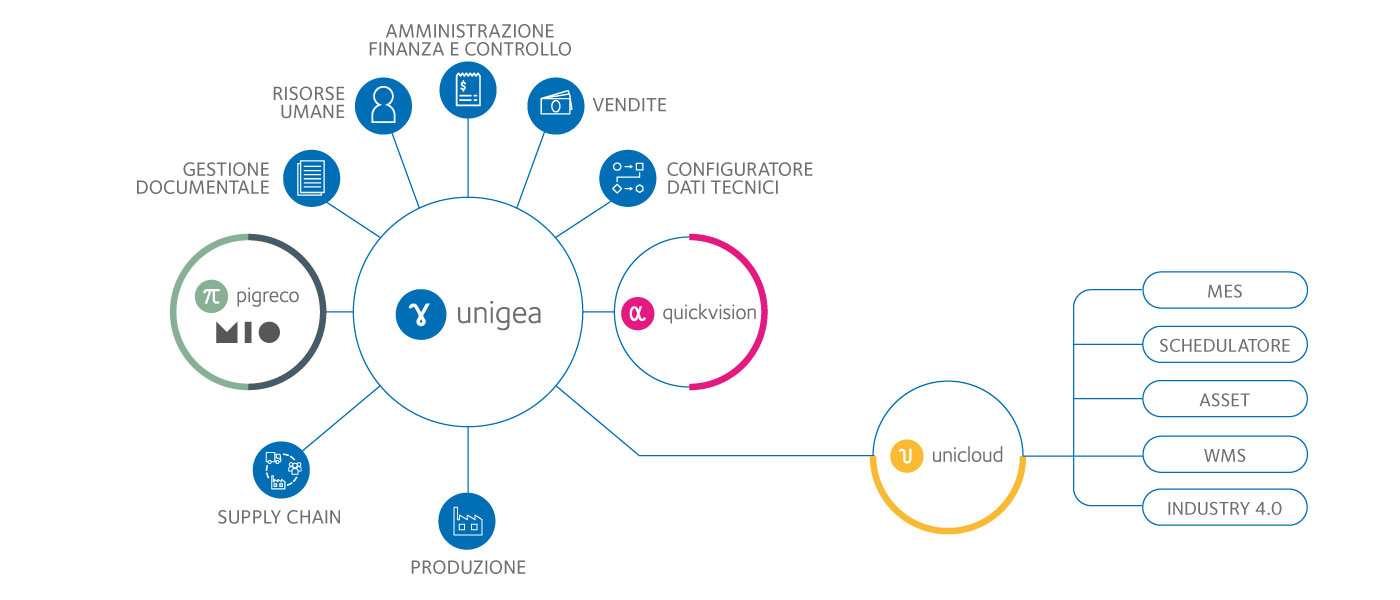
\includegraphics[width=1\textwidth]{soluzioni.jpg}
    \caption{Soluzioni di Deltasystem}
\end{figure}

\clearpage
%% Sottosezione
\subsection{UniCloud}

\begin{wrapfigure}{r}{0.38\textwidth}
    \begin{center}
        
\includegraphics[height=0.06\textheight]{unicloud.png}
    \end{center}
    \caption{Unicloud}
\end{wrapfigure}

%
\includegraphics[scale=0.15]{unicloud.png}

UniCloud è il framework proprietario di deltasystem. Creato per la digital transformation, viene utilizzato per lo svilupo di applicazioni aziendali basate sul cloud. 
La piattaforma facilita l’integrazione e l’estensione delle applicazioni aziendali sul web e su dispositivi mobili, permettendo una gestione dei processi scalabile, la centralizzazione dei dati e un elevata mobilità del software.


%\begin{wrapfigure}{l}{0.38\textwidth}
%    \begin{center}
%        
\includegraphics[width=0.38\textwidth]{unigea.png}
%    \end{center}
%    \caption{Unigea}
%\end{wrapfigure}



%% Sottosezione
\subsection{UniGea}

\begin{wrapfigure}{r}{0.38\textwidth}
    \begin{center}
        
\includegraphics[height=0.06\textheight]{unigea.png}
    \end{center}
    \caption{Unigea}
\end{wrapfigure}




       %% 
\includegraphics[scale=0.15]{unigea.png}


%\noindent
Basato su UniCloud, Unigea è un Erp esteso, cioè in grado di coprire tutte le aree aziendali, e unico, in grado di gestire diverse aree di business da un unica applicazione. Tale modularità permette una configurazione personalizzata in base alle esigenze del cliente.
Unigea, essendo completamente web based, fornisce un ambiente di facile apprendimento ed è accessibile da qualunque piattaforma, indipendentemente dall’hardware (anyclient-anywhere).
L’ERP Unigea è perfettamente integrato con tutte le altre soluzioni offerte da deltasystem.


%% Sottosezione
\subsection{Quickvision}
\begin{wrapfigure}{r}{0.38\textwidth}
    \begin{center}
        
\includegraphics[height=0.06\textheight]{quickvision.png}
    \end{center}
    \caption{Quickvision}
\end{wrapfigure}


%
\includegraphics[scale=0.15]{quickvision.png}

QuickVision è l’applicazione di data analytics per l'analisi interattiva, sintetica e flessibile delle informazioni aziendali, che trasforma in dati visualizzabili graficamente e comodamente navigabili.
Quickvision offre al cliente una piattaforma per consultare dati rapidamente tramite dashboard su misura con livello di dettaglio e filtri configurabili, consentendo quindi a ciascun utente di accedere solo alle informazioni a lui pertinenti.


%% Sottosezione
\subsection{Pigreco}

\begin{wrapfigure}{r}{0.38\textwidth}
    \begin{center}
        
\includegraphics[height=0.06\textheight]{pigreco.png}
    \end{center}
    \caption{Pigreco}
\end{wrapfigure}

%
\includegraphics[scale=0.4]{pigreco.png}

Configuratore tecnico-commerciale ideato per il mondo del mobile e dell'arredamento.
Permette la gestione grafica dell’intero ciclo di vita dell’ordine, dall’acquisizione alla produzione, sia prodotti standard che fuori misura, personalizzati o speciali.
Tale sistema è in grado di recepire le regole aziendali della composizione dei prodotti garantendo il rispetto dei parametri.
Pigreco è inoltre in grado di ottimizzare i flussi e i processi produttivi tramite la generazione di stampe tecniche, schemi di montaggio e liste di lavoro.
Infine Pigreco è dotato di un motore di rendering e un visualizzatore di modelli chiamato MyView.
MyView permette di visualizzare i modelli generati da Pigreco in ambientazioni realistiche e personalizzabili. Questa feature è compatibile con visori 3D per esplorare e analizzare il modello nel dettaglio.

%% Sottosezione
\subsection{MIO}
\begin{wrapfigure}{r}{0.38\textwidth}
    \begin{center}
        
\includegraphics[height=0.06\textheight]{mio.png}
    \end{center}
    \caption{MIO}
\end{wrapfigure}


%
\includegraphics[scale=0.2]{mio.png}

MIO è una piattaforma dedicata alle aziende del settore dell’arredamento nato dall’acquisizione di METAVERSO srl. 
È il primo virtual designer completo per l’arredo-casa.
Pensato per migliorare l’esperienza del cliente, tramite l’utilizzo di tecnologie 3D e realtà aumentata, MIO permette di creare e personalizzare prodotti ed ambienti con modelli ad alta fedeltà.
MIO si integra nativamente con ERP ed e-commerce. Genera ordini con distinta, codici prodotti e rendering, gestisce varianti di prodotto, prezzi e sconti rendendo le informazioni disponibili ai clienti in tempo reale.
Essendo anche MIO web-based ,è accessibile da qualunque browser senza necessità di plugin aggiuntivi. 
Fornisce anche informazioni sulle interazioni e scelte degli utenti per analizzare azioni e strategie di vendita.

\section{Il team}

Durante il mio tirocinio non sono stato inserito in un team. 
I progetti da me realizzati sono stati sviluppati in modo individuale sotto la guida e la supervisione del mio tutor aziendale.


%----------------------------------------------------
%https://www.ibm.com/support/pages/node/6120837#labs
\chapter{Applicazioni utilizzate}
\section{IBM Rational Developer for i}
IBM Rational Developer for i (RDi) è un ambiente di sviluppo integrato(IDE) basato su eclipse, IDE open source di proprietà di Eclipse Foundation.
RDi è ideato specificamente per la programmazione in RPG e COBOL.

%https://www.ibm.com/support/pages/system/files/inline-files/Lab02_RDi_editing%20-%20FreeForm_3.pdf
\subsection{Live Parsing Extensible Editor (LPEX)}
LPEX è l'editor per la scrittura di sorgenti utilizzato da RDi. Rispetto al suo predecessore SEU, LPEX possiede:
\begin{itemize}
    \setlength{\itemsep}{0pt} % Riduce lo spazio tra gli elementi
    \item Editor visuale a colori.
    \item Capacità di aprire più sorgenti in contemporanea.
    \item Visualizzazione della struttura per spostamenti rapidi tra le routine, definizioni di file, variabili ecc.
    \item Creazione guidata di specifiche e procedure.
    \item Controllo della sintassi.
    \item Refactoring.
    \item Tooltip.
    \item Conversione da formato fixed a formato free .
    \item Compatibilità con i comandi di SEU.
    \item Help dotato di manuale RPG.
\end{itemize}

\subsection{Debugger}
RDi è dotato di funzionalità dedicate al debugging tra cui esecuzione passo passo con possibilità di esplorare singole chiamate, monitoraggio delle variabili e delle espressioni in esecuzione e report degli errori.


%https://www.ibm.com/support/pages/system/files/inline-files/Lab01_RDi_intro_2.pdf
\subsection{Remote Systems Explorer (RSE)}
Questo IDE permette un accesso diretto ai file sorgente, tabelle e librerie grazie alla integrazione con IBM i.
Tale integrazione cosente di modificare ed effettuare modifiche del codice da remoto, funzione essenziale per il debugging di programmi web based.



\section{RPGLE}
Report Program Generator Language Enhanced è un'estensione di RPG, un linguaggio di programmazione sviluppato da IBM nel 1958.
Viene utilizzato per lo sviluppo di applicazioni aziendali che operano su sistemi IBM.

\subsection{Caratteristiche "storiche" (RPG)}
Linguaggio compilato, spartano ed essenziale, RPG (Report Program Generator) è ancora oggi è il più compatto fra gli HLL (Linguaggi ad alto livello).
Un programma per aggiornare un campo su tutti i record di un file comprende al massimo quattro istruzioni.

RPG è un linguaggio nato per la produzione di stampe in batch con un flusso di elaborazione strettamente predefinito.
\\
Un programma tipico di stampa prevede un flusso standard:
\begin{itemize}
    \setlength{\itemsep}{0pt} % Riduce lo spazio tra gli elementi
    \item elaborazione dell’intestazione della stampa
    \item elaborazione delle intestazioni delle rotture di livello
    \item elaborazione delle righe di dettaglio
    \item elaborazione dei totali delle rotture di livello
    \item elaborazione dei totali generali della stampa
\end{itemize}
RPG offre pieno supporto a questa modalità di
elaborazione con il “ciclo RPG”, ovvero un comportamento
predefinito da parte del programma in presenza di
determinate istruzioni.


RPG è un linguaggio ‘fortemente tipizzato’, perciò qualunque
elemento a cui il codice fa riferimento (variabile o costante)
deve essere definito espressamente specificandone tipo di
dato e dimensione.
\begin{lstlisting}[language=RPG, caption=Dichiarazione di una variabile alfanumerica di lunghezza 100, label=lst:rpgdeclaration]
    D Message        S             100A         Messaggio di output
\end{lstlisting}


RPG è nato come linguaggio posizionale. Le istruzioni vanno scritte rispettando il cosiddetto “fixed format”, perciò devono rispettare una struttura fissa basata sul significato delle colonne:
\begin{itemize}
    \setlength{\itemsep}{0pt} % Riduce lo spazio tra gli elementi
    \item La riga è lunga 80 caratteri, retaggio delle schede perforate.
    \item Le colonne da 1 a 5 e da 81 in poi non sono riservate e possono essere utilizzate per la scrittura di appunti e commenti
    \item La colonna 6 è riservata all’identificativo della specifica (D per dichiarazioni, C per calcoli ...)
    \item La colonna 7 definisce la presenza di una riga commento tramite l'uso del simbolo *
    \item Il formato delle istruzioni, cioè “cosa scrivere dove”, viene specificato nelle posizioni da 7 a 80,  in base alla tipologia di queste ultime. Il significato delle posizioni da 7 a 80 quindi variano in base alla specifica in uso.
\end{itemize}

\subsection{Caratteristiche moderne (RPGLE)}
Utilizzabile per scrivere programmi interattivi.
\begin{itemize}
    \setlength{\itemsep}{0pt} % Riduce lo spazio tra gli elementi
    \item Pieno supporto dei terminali video e dell’interazione con l’utente
    \item Costrutti semantici più aderenti al paradigma della programmazione strutturata e modulare
    \item Possibilità di realizzare programmi svincolati dal ciclo RPG
    \item Supporto di SQL embedded
\end{itemize}
Totale compatibilità con le versioni precedenti
\begin{itemize}
    \setlength{\itemsep}{0pt} % Riduce lo spazio tra gli elementi
    \item Fino ad oggi anche la versione più recente di RPG accetta e riconosce la sintassi della versione più antica
    \item Struttura delle istruzioni non più (soltanto) fissa
\end{itemize}  
Sono disponibili tre formati:
\begin{itemize}
    \item fixed format: il codice è diviso in colonne e ogni colonna assume un significato diverso.
    A causa della sua scarsa leggibilità e l'avvento del free format, il fixed format non è piu il formato consigliato e viene utilizzato principalmente per il mantenimento dei programmi legacy.
    \begin{lstlisting}[language=RPG, caption=Codice RPG in fixed format, label=lst:rpgfixed]
    CL0N01Factor1+++++++Opcode&ExtFactor2+++++++Result++++++++Len++D+HiLoEq...
    C     IMP           ADD       IVA           TOTALE
    \end{lstlisting}
    \item columnar expression format: simile al fixed format, le istruzioni sono vincolate alle colonne ma offre una maggiore libertà sulla scrittura delle espressioni.
    \begin{lstlisting}[language=RPG, caption=Codice RPG in columnar expression format, label=lst:rpgcolumnar]
    CL0N01Factor1+++++++Opcode&ExtFactor2+++++++Result++++++++Len++D+HiLoEq...
    C                   Eval      Totale = Imp + Iva
    \end{lstlisting}
    \item free format: il codice non è più vincolato alle colonne. Considerato lo standard per la programmazione in RPG, free format offre una maggiore facilità nella lettura del codice, uno stile di programmazione simile ad altri linguaggi di programmazione moderni e una maggiore libertà sull'indentazione del codice.
    \begin{lstlisting}[language=RPG, caption=Codice RPG in free format, label=lst:rpgfree]
    CL0N01Factor1+++++++Opcode&ExtFactor2+++++++Result++++++++Len++D+HiLoEq...
    C/free

    Totale=Imp+Iva;

    C/end-free
    
    \end{lstlisting}
     
\end{itemize} 

Tutti i tipi di formato possono coesistere nello stesso codice purchè correttamente separati.
Fixed e free format utilizzano diversa semantica per definire le specifiche.

\section{DESIGNER Unicloud}
DESIGNER Unicloud è lo strumento che utiliziamo per creare l'interfaccia grafica delle nostre applicazioni.
Il designer è completamente web based e accessibile solo tramite un apposito link riservato agli sviluppatori.
Come molti editor dedicati alle interfacce grafiche, il designer di unicloud permette l'inserimento di diverse risorse.

\subsection{Risorse}
Le risorse sono componenti di un form con attributi preconfigurati.
Possiamo raggrupparli in
\begin{itemize}
    \item elementi di input (bottoni semplici, radiali, checkbox, caselle di testo, select box, date picker ...)
    \item elementi testuali (lable, link)
    \item elementi multimediali (immagini, video, grafici, mappe)
    \item elementi strutturali (tabelle, celle, pannelli)
    \item elementi prefabbricati (form)
\end{itemize}

\subsection{attributi}
Ogni risorsa non è altro che un elemento dotato di specifici attributi.
Tramite la modifica di questi attributi, possiamo trasformare una risorsa in qualunque modo desideriamo.
Queste modifiche possono essere semplici variazioni estetiche come dimensioni, carattere, colore e allineamento, oppure 
modifiche alla funzione come visibilità, sola lettura, abilitazione dell'elemento, tipo di dato contenuto e riferimenti al database.
è possibile modificare questi attributi in esecuzione e sarà importante per i requisiti del nostro programma.

\subsection{scheletro}
Per poter interagire con l'interfaccia dobbiamo prima costruire lo scheletro tramite l'apposito menu. 
Lo scheletro consiste in 2 file.
Il primo, il file RPGLE, sarà il file dove avveine la programmazione
il secondo, il file DSPF, contiene una lista di tutti i campi di input presenti nel progetto e il loro tipo (definito dagli attributi del relativo campo di input). 
Questo file viene richiamato dal file RPGLE per poter ricavare i valori dei campi dell'interfaccia durante l'esecuzione.
Entrambi i file vengono generati con tutti gli elementi necessari e la struttura del flusso di esecuzione.
Come dice il nome questo è uno scheletro e sarà nostra responsabilità riempire il programma affinchè l'interfaccia del designer si comporti come richiesto.

\section{Quickvision}
QuickVision è il programma che utiliziamo per costruire e mostrare i dati tramite interfacce personalizzate.
Sarà possibile creare:

\begin{itemize}
    \item tabelle semplici
    \item tabelle interattive
    \item filtri dinamici locali e globali
    \item campi di ricerca
    \item grafici semplici
    \item grafici dinamici
    \item scorciatoie a tabelle più specifiche
    \item conversione di dati in codici a barre e/o QR
\end{itemize}

Possiamo visualizzare queste tabelle e grafici singolarmente oppure possiamo mostrarle in un unico pannello di controllo chiamato "schema".

Il vantaggio di uno schema sta non solo nel poter visualizzare piu elementi in contemporanea senza navigare costantemente, ma anche nel poter interagire con più tabelle e grafici all'unisono.
Per esempio posso filtrare una tabella per un determinato valore e i grafici e tabelle ad essa collegata vengono aggiornate in tempo reale con i nuovi valori.

Il risultato finale sarà un pannello di controllo a cui accedere alle informazioni opportunamente organizzate come richiesto dal cliente

Il progetto è definito da un file xml.


\section{Database}
Tutti i progetti sono stati realizzati usando un database di test.
Il database di test è una copia esatta del database aziendale perciò le tabelle sono identiche in quanto struttura ma conterranno dati fittizi e/o obsoleti.

I primi 6 campi di ogni tabella sono riservati alle informazioni riguardo l'utente la data e l'ora dell'immissione e dell'ultimo aggiornamento del record

\subsection{Tabelle dei progetti di apprendimento}
ANGCF00F si occupa di immagazzinare le informazioni anagrafiche dei clienti e dei fornitori. 
\\Tra le informazioni disponibili sono presenti nome, indirizzo, ragione sociale, partita iva, telefono, fax, e-mail.
\\I record sono identificati dal codice cliente fornitori
\\
\\ANGFL00F viene utilizzata per recuperare informazioni riguardo una determinata filiale come indirizzo, ragione sociale, telefono e email.
\\La filiale è identificata dal codice filiale FLCDFL
\\Il campo FLCDCF contiene la chiave esterna del cliente/fornitore a cui questa filiale è associata.
\\
\\OCLGT00F e OFRAT00F sono le tabelle contenenti le informazioni di testata degli ordini dei clienti e dei fornitori rispettivamente.
\\I singoli ordini sono identificati dall'anno e dal numero dell'ordine. 
\\L'azienda assenga un numero progressivo a ogni ordine che si azzera con l'inizio del nuovo anno.
\\Questa tabella ci permette di accedere a diverse caratteristiche dell'ordine, in particolare lo stato dell'ordine, l'evasione, le date di richiesta, consega prevista, tipo di ordine e causale.
\\
\\OCLGD00f e OFRAD00F contengono i singoli articoli degli ordini dei clienti e dei fornitori. 
\\Vengono identificati dal loro codice articolo e il riferimento alla riga cel cliente o fornitore.
\\La tabella contiene informazioni riguardanti i singoli articoli come descrizione, peso dell'articolo, volume, dimensioni, quantità ordinata, in spedizione e spedita
\\
\\TBBSE00F contiene le descrizioni di ogni tabella del database dato il codice del record di interesse.
\\Ogni tabella è identificata da 4 campi che descrivono il nome della tabella diviso nelle sue componenti:
\begin{itemize}
    \item TBPRFS prefisso della tabella
    \item TBCTB1 primo codice tabella
    \item TBCTB2 secondo codice tabella
    \item TBCTB3 terzo codice tabella
\end{itemize}


\subsection{Tabelle progetto finale}
GSTGAS00V contiene i giustificativi delle giornate di assenza. In questa tabella sono racchiusi tutte le richieste di permesso identificate da un codice.
\\Ogni record ha come chiavi esterne gli identificatifi della risorsa che usufruisce dell'assenza, dell'azienda della risorsa e del giustificativo assenza.
\\Se un assenza dura piu di un giorno allora esisterà un record per ciascuna giornata ogniuno con riferimento allo stesso giustificativo assenza.
\\Da questa tabella possiamo inoltre ricavare la data di assenza (nel caso di assenza di piu giorni saranno elencati i singoli giorni), l'ora di inizio e fine assenza (nulli nel caso di assenza di piu giorni) e i minuti di assenza.
\\Si può notare che queta tabella non è il file originale ma una vista. Si capisce ciò dal suffisso V nel nome del file. 
\\
\\GSTASS00F contiene i giustificativi delle assenze individuali.
\\In questa tabella abbiamo accesso a piu dettagli riguardanti l'assenza di una risorsa.
\\Ogni record è identificato da un codice identificativo.
\\Le informazioni di nostro interesse da questa tabella sono la data di inizio e termine dell'assenza, lo stato dell'autorizzazione e la causale.
\\
\\GRTANG00F contiene un elenco di tutte le possibili causali di un assenza.
\\Questa tabella è di nostro interesse per poter distinguere il tipo di una causale, in particolare se identifica ferie o permessi.
\\
\\DBQANG00F è la tabella dei qualificatori. Dato il nome di una tabella e la colonna si possono ricavare il tipo, la descrizione e le note tecniche di quel campo.
\\
\\CDRAZN00F contiene il calendario aziendale. Verrà utilizzata solo per ricavare l'ultima data possibile del calendario per il controllo degli errori.
\\
\\PRECNS00F contiene la data di chiusura del consuntivo. Non mi sono state fornite altre informazioni a riguardo. Viene utilizzata per effettuare il controllo degli errori.


%-----------------------------------------------------------------------------------------------------------------------

\chapter{Progetti di apprendimento}
\section{Scopo}
Durante il tirocinio sono stati completati un totale di tre progetti.
I primi due progetti sono stati svolti al fine di conoscere l'ambiente di sviluppo, imparare il linguaggio utilizzato e prendere dimestichezza con gli strumenti forniti.
Il terzo è il progetto principale e verrà analizzato nel capitolo seguente.

\section{ST2, schermata di gestione di clienti e fornitori tramite gestionale unigea}
Il primo progetto consiste nella realizzazione di un programma per la visualizazione delle informazioni riguardanti clienti e fornitori.

Da questa lista si potranno mostrare tramite interfacce aggiuntive le informazioni riguardanti uno specifico cliente/fornitore, gli ordini ad esso relativi (divisi per ordini cliente e ordini fornitore) e le sue filiali qualora ne fosse in possesso.

I dettagli del cliente/fornitore sono modificabili tramite un apposita schermata che si apre da un pulsante collocato a lato del pannello.

Infine è possibile modificare o aggiungere nuove filiali sempre tramite un apposito pulsante.

\subsection{Diagramma dei casi d'uso}
Possiamo rappresentare le funzioni del programma sottoforma di un diagramma dei casi d'uso come segue:

\begin{figure}[H]
    \centering
    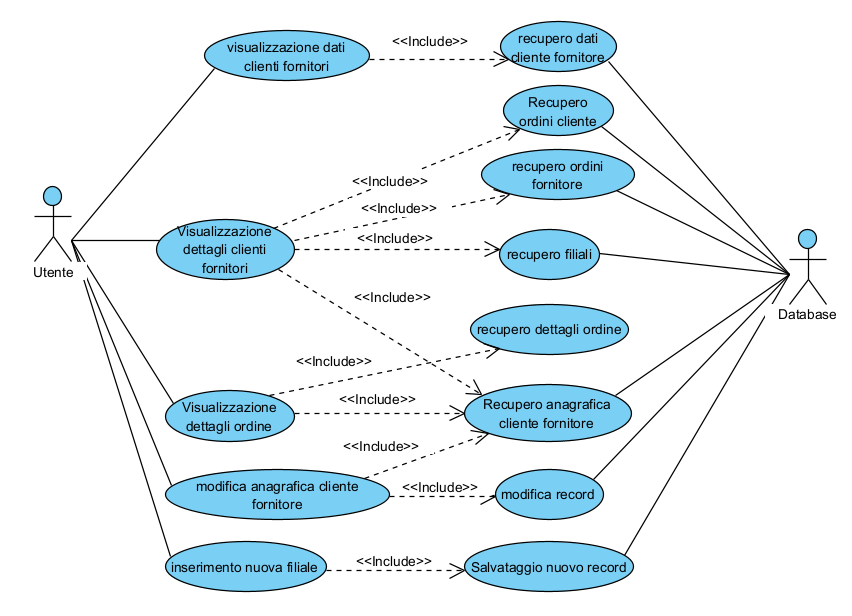
\includegraphics[width=0.6\textwidth]{diagrammi/caso d'uso 1.png}
    \caption{Cartella dei progetti}
\end{figure}

\subsection{Diagramma di stato}
Tramite un diagramma di stato possiamo rappresentare il flusso dei programmi.
Consideriamo come stato la schermata correntemente attiva.

\begin{figure}[H]
    \centering
    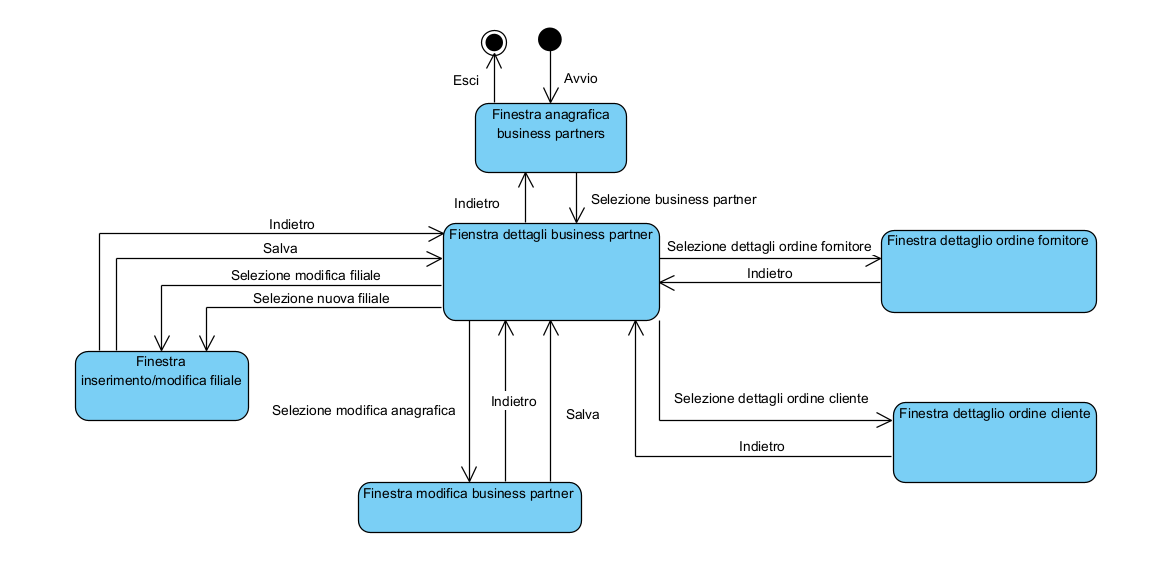
\includegraphics[width=\textwidth]{diagrammi/state progetto 1.png}
    \caption{Cartella dei progetti}
\end{figure}

\subsection{Flusso del programma}
I programmi in rpgle vengono creati con uno scheletro già pronto all'uso in base alla configurazione grafica della schermata.
Questo scheletro è preimpostato per seguire un determinato flusso prestabilito dall'azienda.
Questo flusso non deve essere mai modificato. Possono essere aggiunte funzioni all'interno delle opportune funzioni del flusso ma il flusso stesso deve rimanere invariato.
Tutti i programmi rpgle useranno lo stesso flusso rappresentato in nel seguente activity diagram:

\begin{figure}[H]
    \centering
    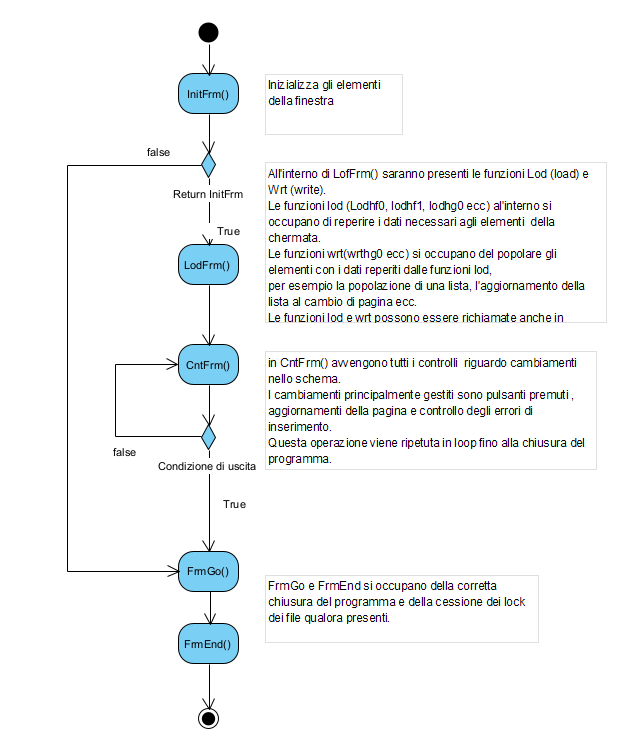
\includegraphics[width=0.7\textwidth]{diagrammi/flusso.png}
    \caption{Flusso dei programmi rpgle specificato dall'azienda}
\end{figure}

\subsection{Struttura del programma}
Il nostro progetto è composto di 6 interfacce e un egual numero di programmi che le gestiscono.
I programmi sono nominati con il prefisso ST2, codice che identifica l'ambiente dedicato agli stagisti numero 2, e un numero incrementale.
La numerazione parte da 010 poiché un programma 000 già esisteva allo scopo di ambiente di prova.


Come da standard aziendali, ogni programma deve rispettare un rigido ciclo prefissato.
Tale ciclo è già predisposto al momento della creazione dello scheletro.
Le uniche modifiche che possiamo apportare sono all'interno delle operazioni lod (funzioni di caricamento), wrt (funzioni di scrittura) e cnt (funzioni di controllo) dei singoli elementi delll'interfaccia.



\subsection{ST2010}
ST2010 è la schermata principale del nostro programma.
In questa schermata vengono visualizzata una lista di clienti e fornitori chiamata "business partners".
\\Oltre a mostrare le informazioni principali di un business partner (id, ragione sociale e indirizzo), Il programma anticipa all'utente la presenza di dati riguardanti le filiali di quel partner tramite un icona gialla.
\\Sono presenti in un apposito menu laterale, 3 pulsanti che filtrano la tabella per clienti, fornitori o tutti.

\begin{figure}[H]
    \centering
    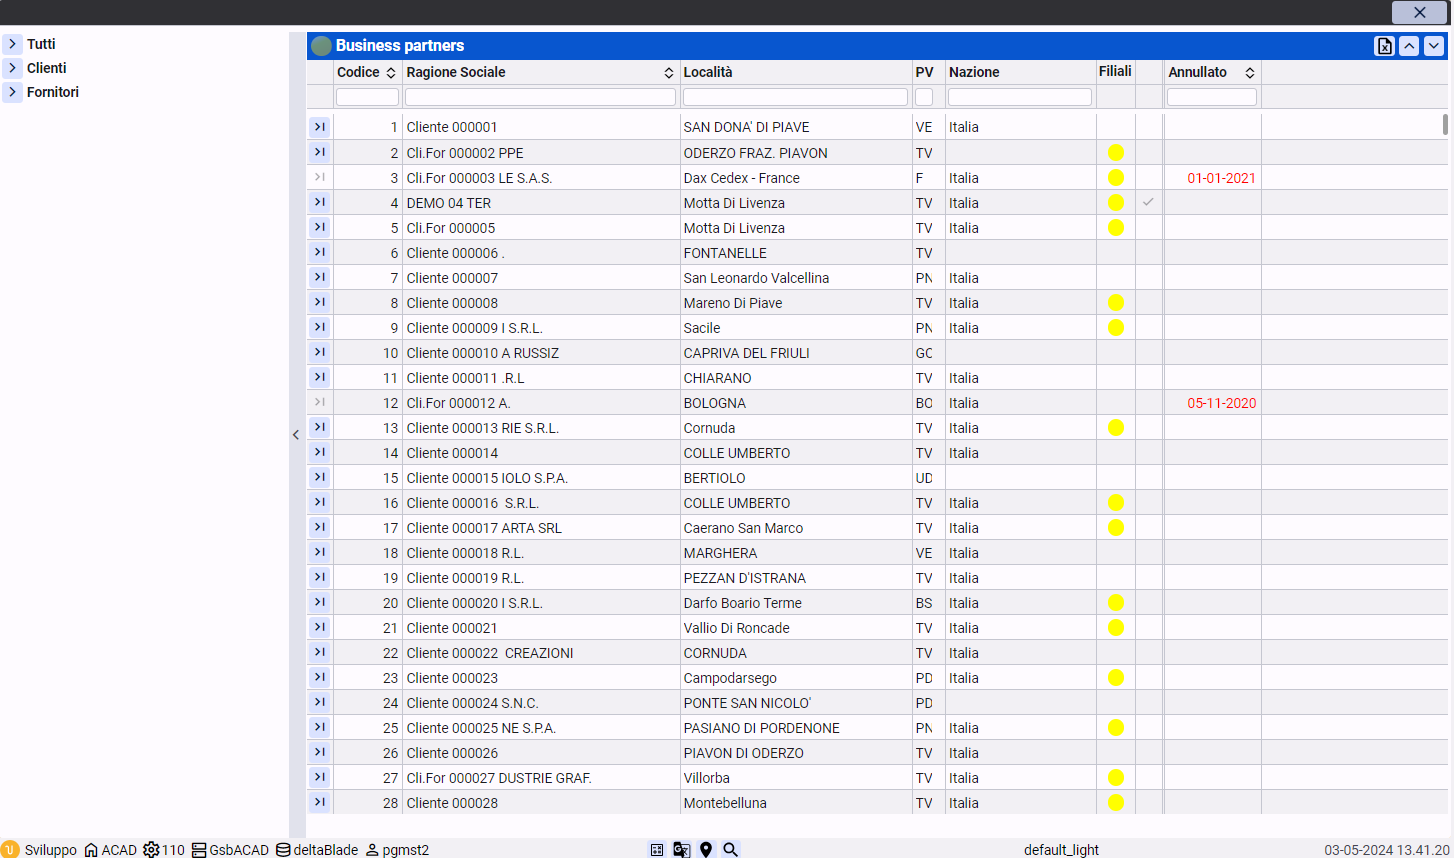
\includegraphics[width=0.9\textwidth, trim=0cm 0cm 0cm 0cm, clip]{st2/ST2010.png}
    \caption{Schermata ST2010}
\end{figure}

\begin{figure}[H]
    \centering
    \includegraphics[width=0.9\textwidth, trim=0cm 0cm 0cm 0cm, clip]{st2/struttura ST2010.png}
    \caption{Struttura della schermata ST2010}
\end{figure}


%\begin{figure}[H]
%    \centering
%    \begin{minipage}{0.45\textwidth}
%        \centering
%        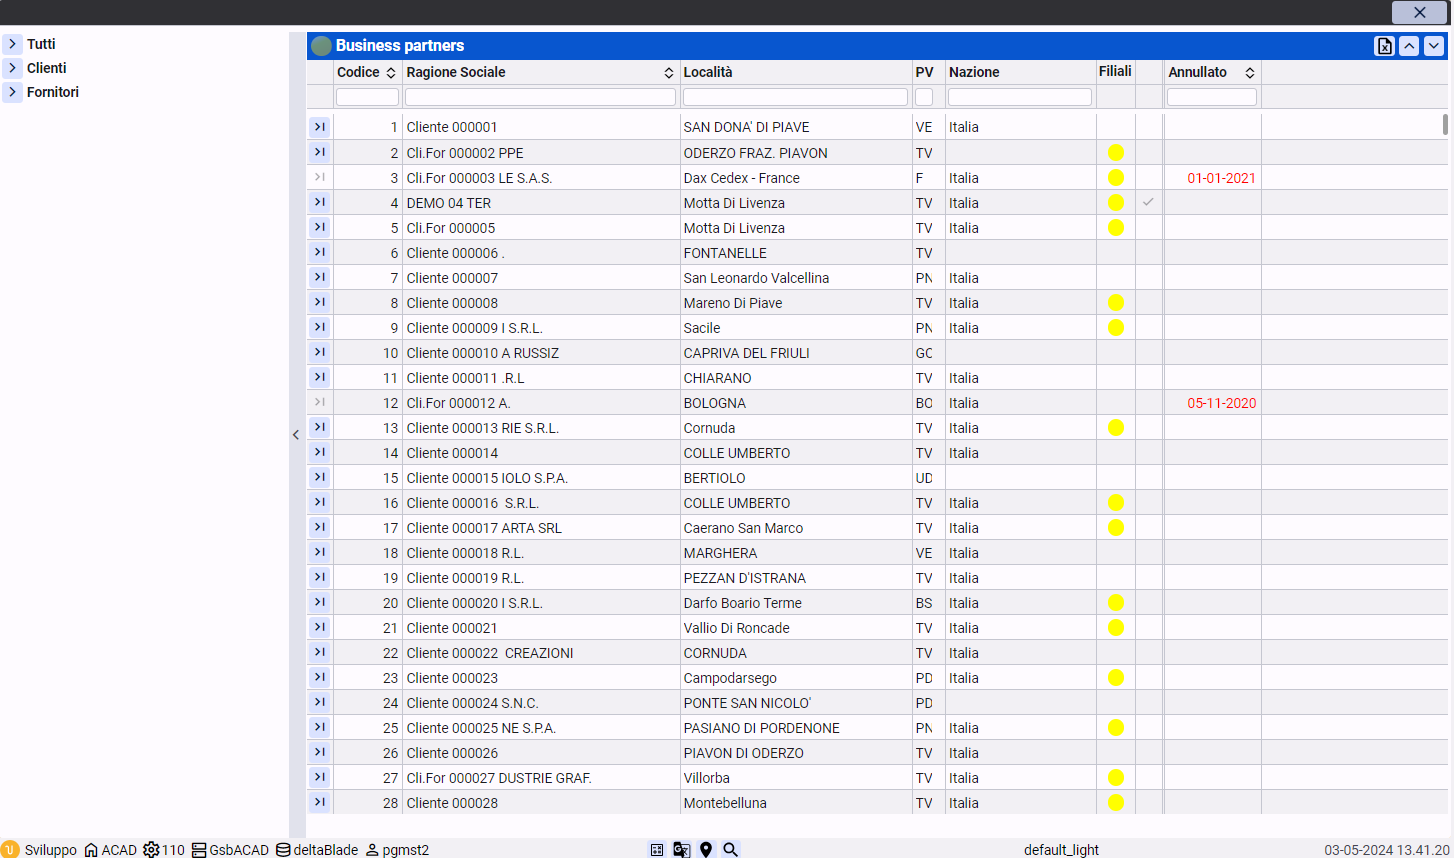
\includegraphics[ height=0.2\textheight]{st2/ST2010.png}
%        \caption{Schermata ST2010}
%    \end{minipage}
%    \hfill
%    \begin{minipage}{0.45\textwidth}
%        \centering
%        \includegraphics[height=0.2\textheight]{st2/struttura ST2010.png}
%        \caption{Struttura della schermata ST2010}
%    \end{minipage}
%\end{figure}

\subsection{ST2011}
ST2011 si occupa della visualizzazione dei dettagli realtivi al business partner selezionato in ST2010, le sue filiali (se esistono) e i suoi ordini divisi per ruolo (ordini cliente e ordini fornitore).
Questa schermata permette di:
\begin{itemize}
    \item Visualizzare i dettaglio del business partner come indirizzo, ragione sociale e partita IVA.
    \item Possibilità di modificare il contenuto tramite l'apposito pulsante a lato della tabella. Tale pulsante apre la schermata ST2012 che si occuperà della modifica.
    \item Visualizzare una lista delle filiali esistenti. Vengono mostrati ragione sociale indirizzo e numero di telefono se esiste.
    \item Possibilità di inserire nuove filiali, qualora necessario, tramite l'utilizzo della schermata ST2014. La schermata viene aperta tramite un apposito pulsante nell'intestazione della tabella.
    \item Possibilità di modificare una filiale tramite la schermata ST2014. L'apposito pulsante si trova all'inizio della riga scelta.
    \item Visualizzare una lista degli ordini cliente e di ordini fornitore (selezionabili solo se il busines partner rientra nella categoria). 
    Vengono mostrati numero di ordine e anno di richiesta (che identificano il singolo ordine) seguiti da data dell'ordine, data di richiesta consegna, il riferimento e lo stato di evasione dell'ordine. 
    Quest'ultimo è rappresentato da un bollino colorato di rosso per ordini non evasi, giallo se evasi parzialmente e verde se completamente evasi.
    \item Possibilità di espandere i dettagli dell'ordine aprendo ST2015 e ST2016 rispettivamente. L'apertura di queste schermate avviene tramite un pulsante presente nella prima colonna di ogni record.
\end{itemize}

\begin{figure}[H]
    \centering
    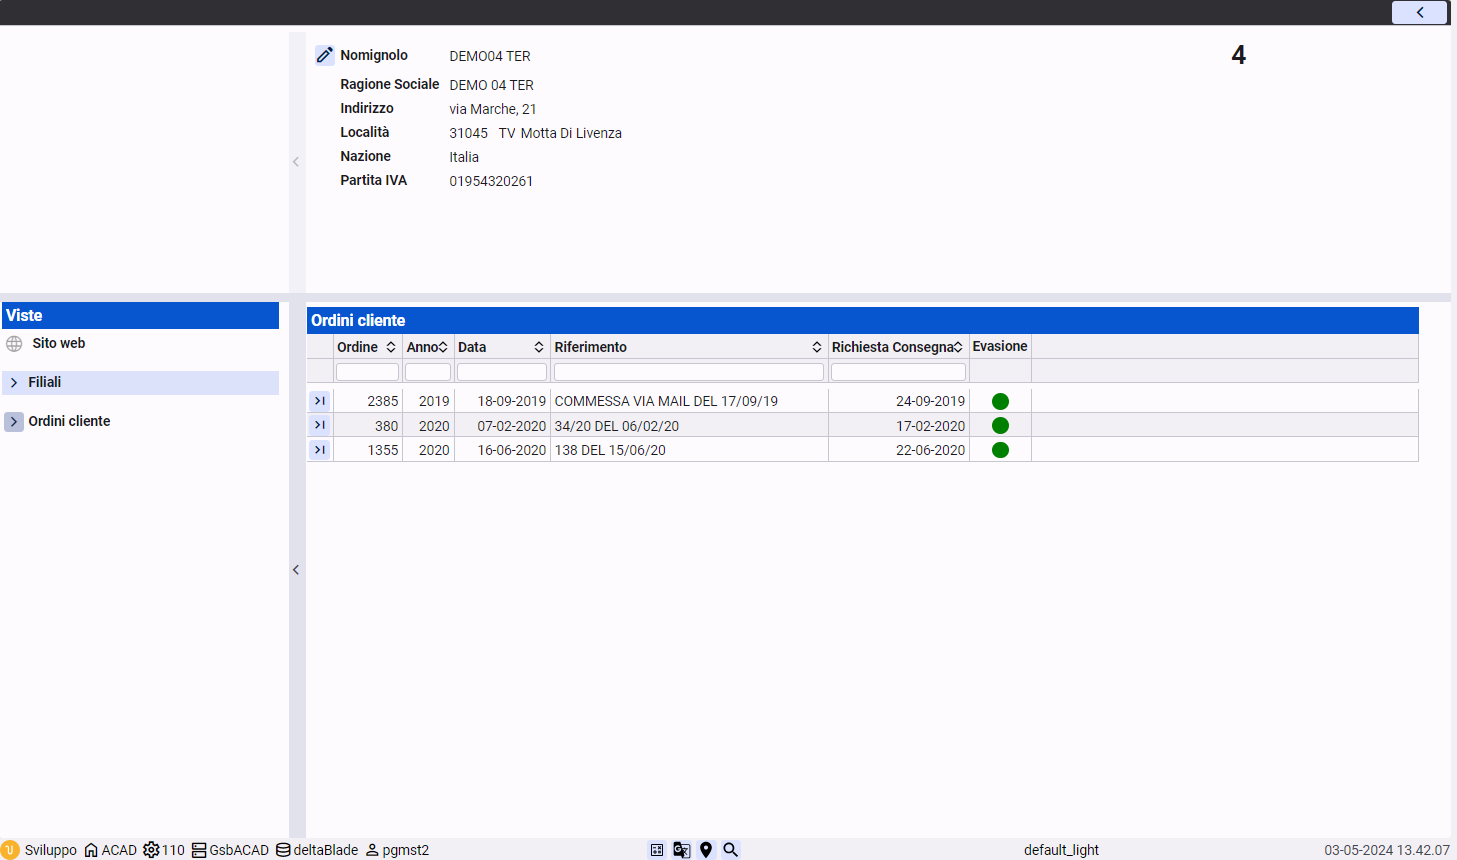
\includegraphics[width=0.9\textwidth, trim=0cm 0cm 0cm 0cm, clip]{st2/ST2011 ordini.png}
    \caption{Schermata ST2011 con lista ordini cliente}
\end{figure}

\begin{figure}[H]
    \centering
    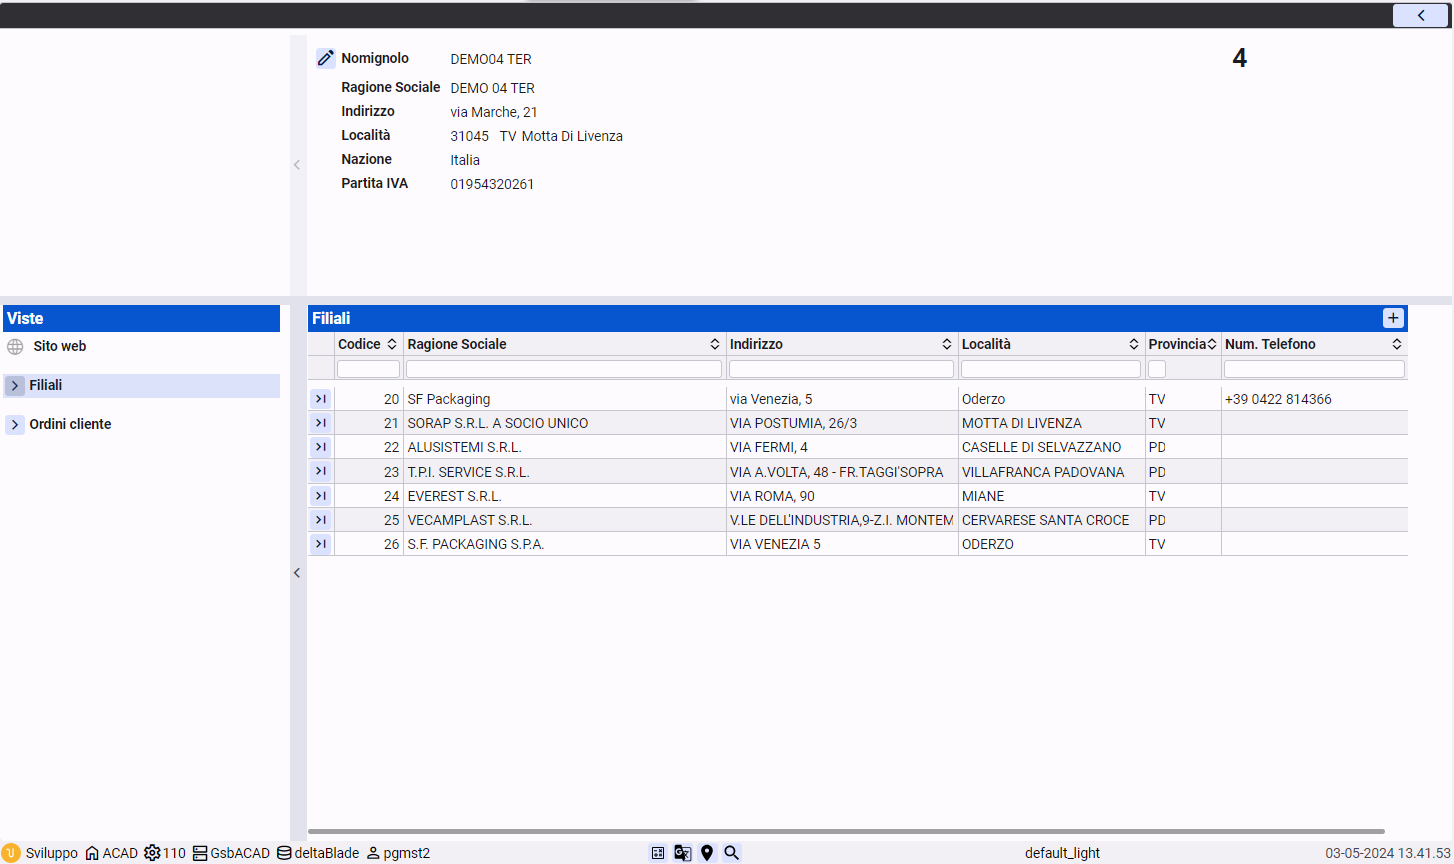
\includegraphics[width=0.9\textwidth, trim=0cm 0cm 0cm 0cm, clip]{st2/ST2011 filiali.png}
    \caption{Schermata ST2011 con lista delle filiali}
\end{figure}



\subsection{ST2012}
ST2012 contiene tutti i campi di testo necessari per la modifica dei dati di un cliente/fornitore.
Questi campi vengono precompilati con le informazioni correnti del business partner da modificare per aggevolare l'inserimento di modifiche da parte dell'utente

\begin{figure}[H]
    \centering
    \begin{minipage}{0.45\textwidth}
        \centering
        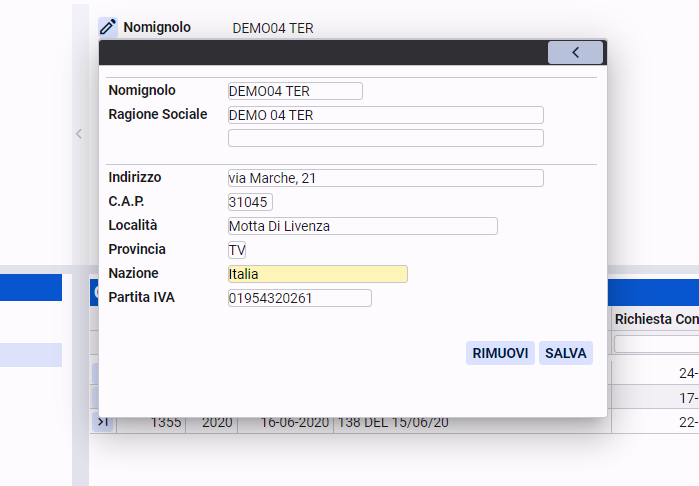
\includegraphics[ height=0.25\textheight]{st2/ST2012.png}
        \caption{Schermata ST2012}
    \end{minipage}
    \hfill
    \begin{minipage}{0.45\textwidth}
        \centering
        \includegraphics[height=0.25\textheight]{st2/struttura ST2012.png}
        \caption{Struttura della schermata ST2012}
    \end{minipage}
\end{figure}

\subsection{ST2014}
ST2014 è la schermata dedicata all'inserimento o modifica dei dati di una nuova filiale. 
I campi di testo sono tutti editabili ad eccezione dei primi 2 contenenti la descrizione del business partner a cui viene associata la filiale.

\begin{figure}[H]
    \centering
    \begin{minipage}{0.45\textwidth}
        \centering
        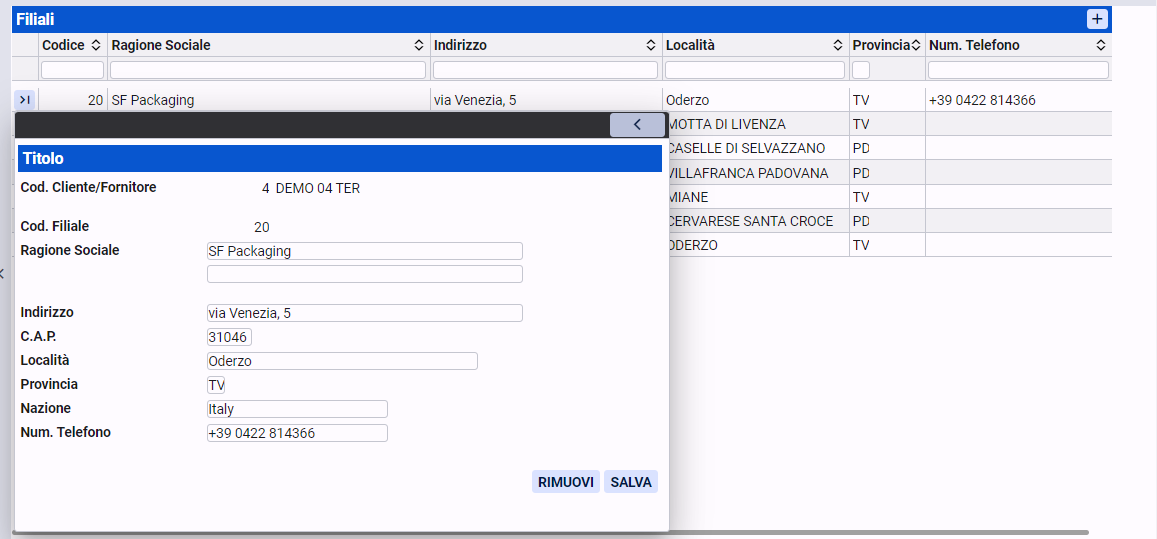
\includegraphics[ height=0.22\textheight, trim=0.5cm 0cm 13cm 3.5cm, clip]{st2/ST2014.png}
        \caption{Schermata ST2014 per modifica di una filiale}
    \end{minipage}
    \hfill
    \begin{minipage}{0.45\textwidth}
        \centering
        \includegraphics[height=0.22\textheight]{st2/struttura ST2014.png}
        \caption{Struttura della schermata ST2014}
    \end{minipage}
\end{figure}

\subsection{ST2015 e ST2016}
ST2015 e ST2016 sono le schermate che mostrano i dettagli di un ordine, il suo stato, chi lo ha commissionato e una lista dei singoli prodotti ordinati.
Le due schermate si differenziano per le diverse informazioni riguardante l'ordine mostrate.

Nel caso di "cliente" viene mostrato il riferimento dell'ordine mentre nel caso di "fornitore" vengono mostrati il tipo e la causale.

\begin{figure}[H]
    \centering
    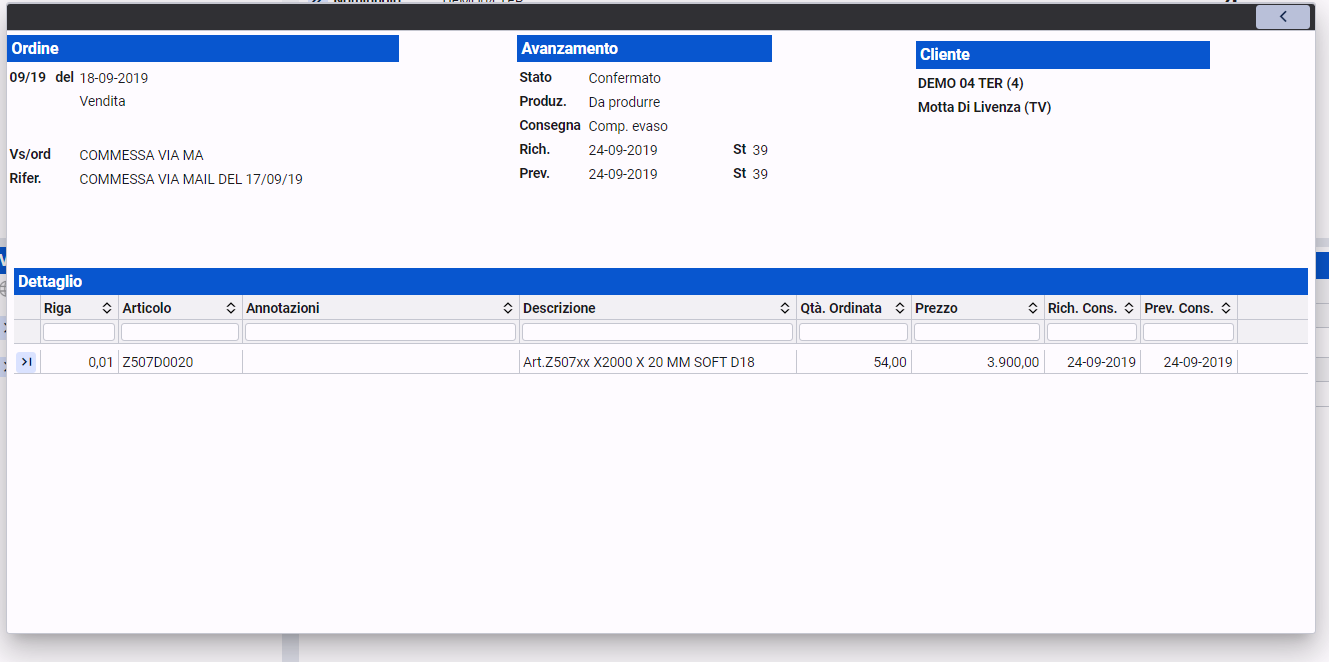
\includegraphics[width=0.9\textwidth, trim=0cm 0cm 0cm 0cm, clip]{st2/ST2015.png}
    \caption{Schermata ST2015}
\end{figure}

\begin{figure}[H]
    \centering
    \includegraphics[width=0.9\textwidth, trim=0cm 0cm 0cm 0cm, clip]{st2/struttura ST2015.png}
    \caption{Struttura della schermata ST2015}
\end{figure}


\newpage
%-----------------------------------------------------------------------------------------------------------




\section{Progetto 2, visualizzazione interattiva degli ordini tramite l'utilizzo di quickvision}
Il secondo progetto prevede l'uso di quickvision per la realizzazione di un pannello di controllo contenente informazioni riguardanti gli ordini dell'azienda e informazioni derivate. 
Sarà possibile inoltre visualizzare i dati della tabella sottoforma di grafici, aprire le tabelle contenenti dettagli riguardo specifici ordini e applicare filtri globali.

Poiché è stato utilizzato quickvision, non è stato scritto codice per il funzionamento del progetto.
Ogni grafico e tabella è il risultato di un lavoro di configurazione dell'ambiente.

\begin{figure}[H]
    \centering
    \includegraphics[width=\textwidth, trim=0cm 0cm 0cm 0cm, clip]{quickvision/tabella nazioni proprietà.png}
    \caption{Ambiente di lavoro quickvision}
\end{figure}

\subsection{Preparazione del progetto}

\begin{wrapfigure}{r}{0.5\textwidth}
    \centering
    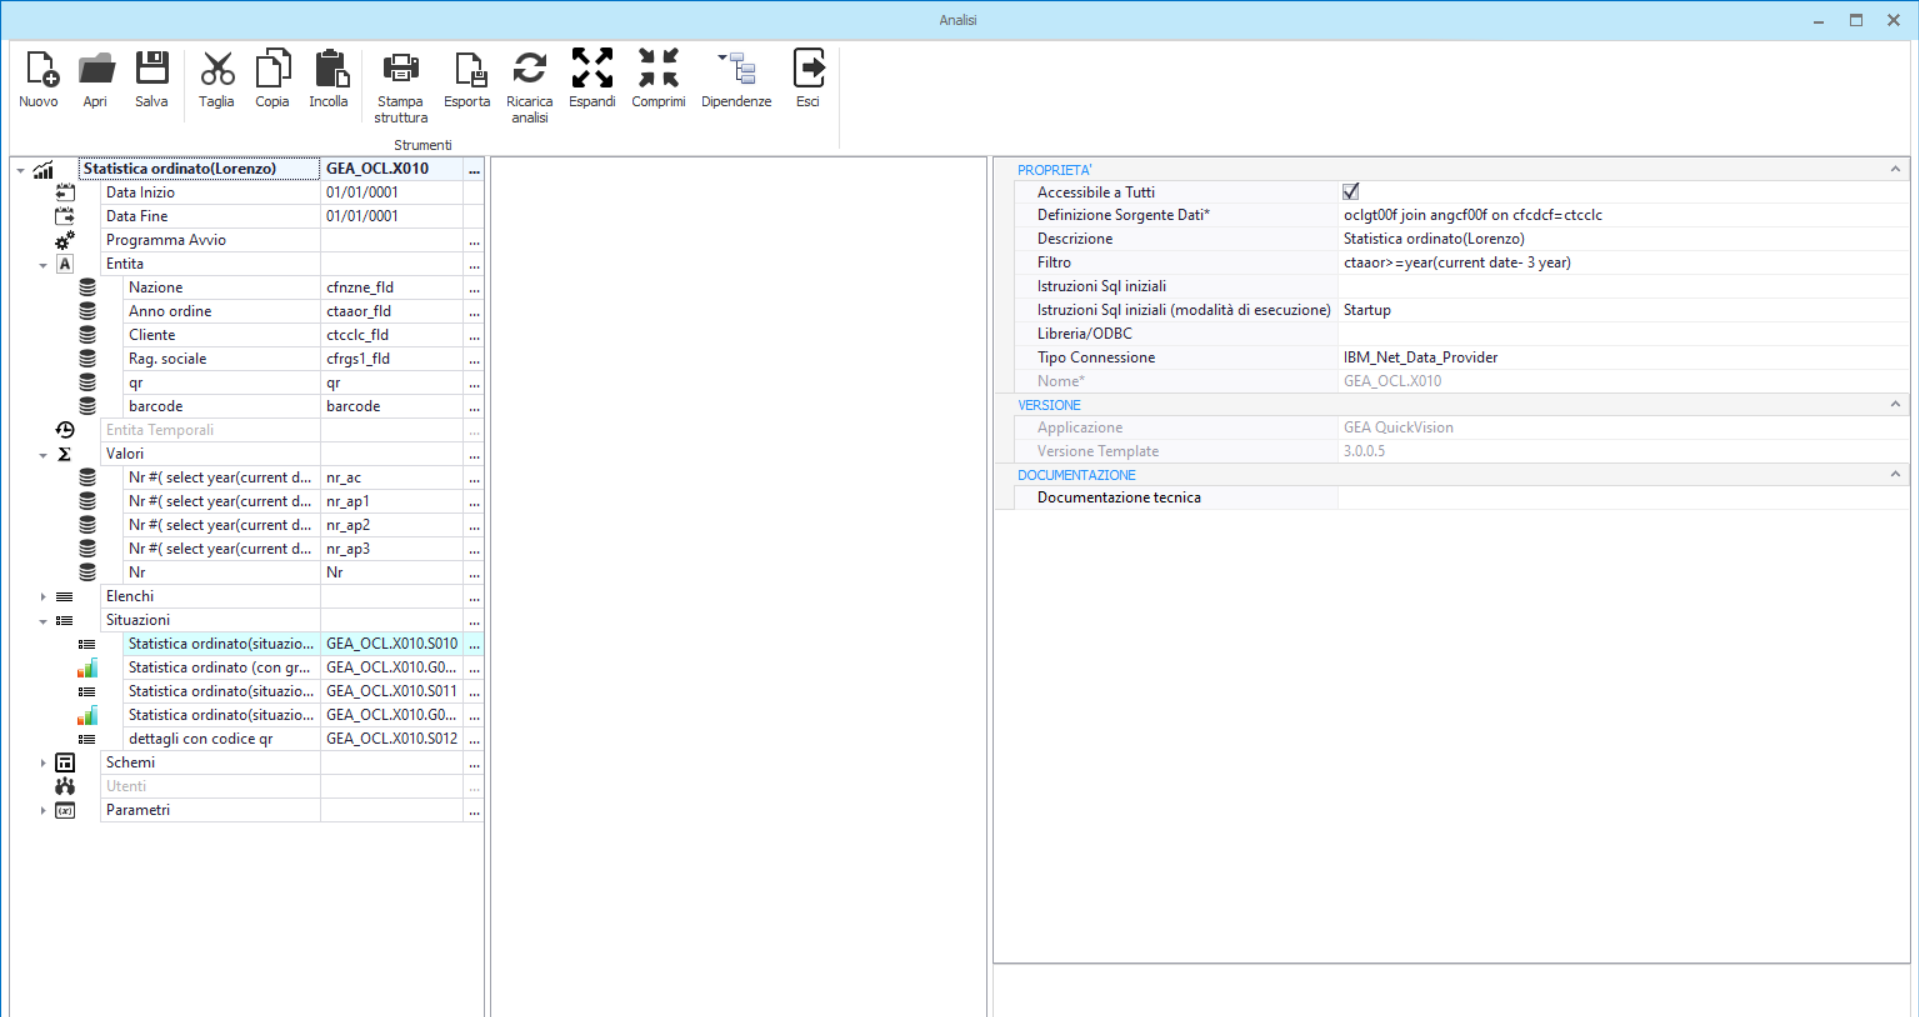
\includegraphics[width=0.5\textwidth, trim=26cm 13cm 0cm 4cm, clip]{quickvision/pannello di configurazione progetto.png}
    \caption{Definizione sorgente dati}
\end{wrapfigure}

Prima di poter creare il pannello di controllo bisogna preparare l'ambiente.
L'elemento fondamentale di un pannello in quickvision è la sorgente dei dati.
Questo campo va compilato come il "FROM" di una richiesta SQL.
La nostra sorgente sarà un unione tra le tabelle di anagrafica clienti/fornitori (angcf00f) e testata ordini clienti (oclgt00f).
L'intero progetto farà riferimento a questa sorgente.

Dalle proprietà del progetto è possibile definire un filtro, come il "WHERE" in SQL, da applicare alla sorgente. 
In questo caso vengono selezionati gli ordini degli ultimi 3 anni.
\newpage
\subsection{Entità}

\begin{wrapfigure}{r}{0.5\textwidth}
    \centering
    \includegraphics[width=0.5\textwidth, trim=26cm 0cm 0cm 4cm, clip]{quickvision/entità nazione.png}
    \caption{Proprietà di un entità}
\end{wrapfigure}
Le entità sono i campi che le tabelle e i grafici useranno.
Anche le entità necessitano di una sorgente dati. Nel loro caso la sorgente sarà il campo di cui vogliono assumere il valore oppure una richiesta piu complessa.
Per esempio l'entità \textbf{nazione} potrebbe essere una diretta rappresentazione del campo cfnzne (nazione del cliente) ma poichè è possibile la presenza di campi nulli modifichiamo la fonte con la seguente richiesta:
case when trim(cfnzne)='' then 'non definita' else cnfzne end.
Con questa aggiunta l'utente non vedrà campi vuoti al momento della visualizzazione.

Le entità possono assumere la forma di codici a barre e codici QR tramite un apposita opzione nelle proprietà dell'entità stessa.

Infine è necessario dichiarare il tipo di variabile utilizzata affinche quickvision possa interpretarla a dovere.



%\subsection{Valori}
%I valori sono elementi che non ricavano le informazioni dalla sorgente dati e sono esclusivamente valori numerici.
%
%Possono essere utilizzate per operazioni di filtraggio.
%Per esempio possiamo dichiarare un valore per gli ordini dell'anno corrente come "sum(case when ctaaor=year(current date) then 1 else 0)".
%
%\begin{figure}[h]
%    \centering
%    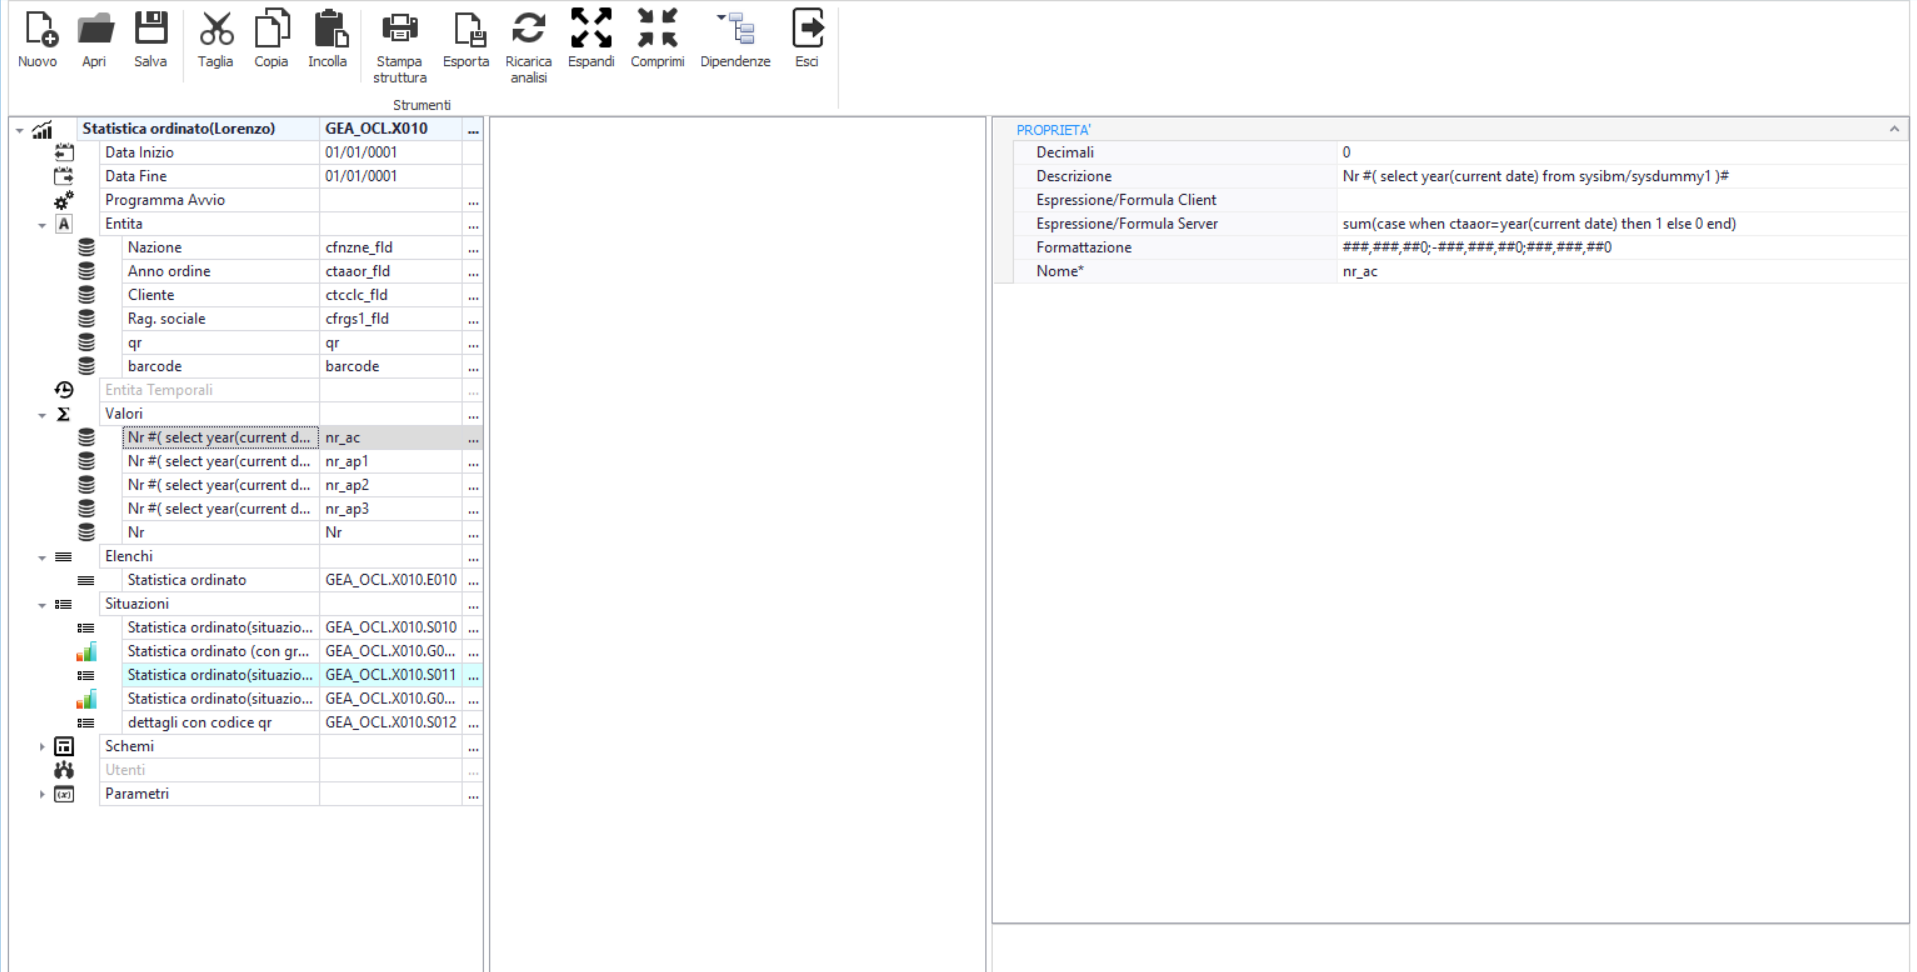
\includegraphics[height=0.1\textheight, trim=26cm 17cm 0cm 3cm, clip]{quickvision/valore.png}
%    \caption{Proprietà di un valore}
%\end{figure}
%\newpage

\subsection{Configurazione di tabelle e grafici}
La configurazione di una tabella avviene tramite l'inserimento delle entità configurate precedentemente negli assi x e y.
Dalle proprietà della tabella è possibile modificarne l'aspetto, come dimensione del testo e colore delle celle, o abilitare certe funzioni come la barra di filtraggio, l'esportazione in excel e le abilitazioni per l'accesso.
Nel caso del colore delle celle è possibile configurarlo in modo tale da associare i colori in base alla circostanza.
Nel progetto realizzato i valori inferiori a 5 sono colorati di rosso, quelli uguali a 5 di grigio e quelli maggiori di 5 di verde.

Posso predisporre le tabelle all'apertura di altre tabelle sottoforma di finestra popup.
In questo modo posso, alla pressione di un icona nella tabella, visualizzare un'ulteriore tabella contenente i dettagli della mia selezione.
Tale collegamento viene definito \textbf{relazione} nel pannello di configurazione.

Le tabelle del nostro grafico sono 3:
\begin{enumerate}
    \item Statistica ordinato, tabella del numero di ordini all'anno divisi per nazione. Tramite l'apposito pulsante viene aperta una tabella "Statistica ordinato per clienti" filtrata per la nazione selezionata.
    \item Statistica ordinato per clienti, tabella del numero di ordini all'anno divisi per cliente. La tabella viene richiamata da "Statistica ordinato". Tramite l'apposito pulsante viene aperta la tabella "Dettagli con codice qr" filtrata per l'utente selezionato.
    \item Dettagli con codice qr, tabella contenente le informazioni dei clienti e la conversione del loro id in codice a barre e codice qr. Viene richiamata dalla tabella "Statistica ordinato per clienti".
\end{enumerate}


\begin{figure}[H]
    \centering
    \begin{minipage}{0.45\textwidth}
        \centering
        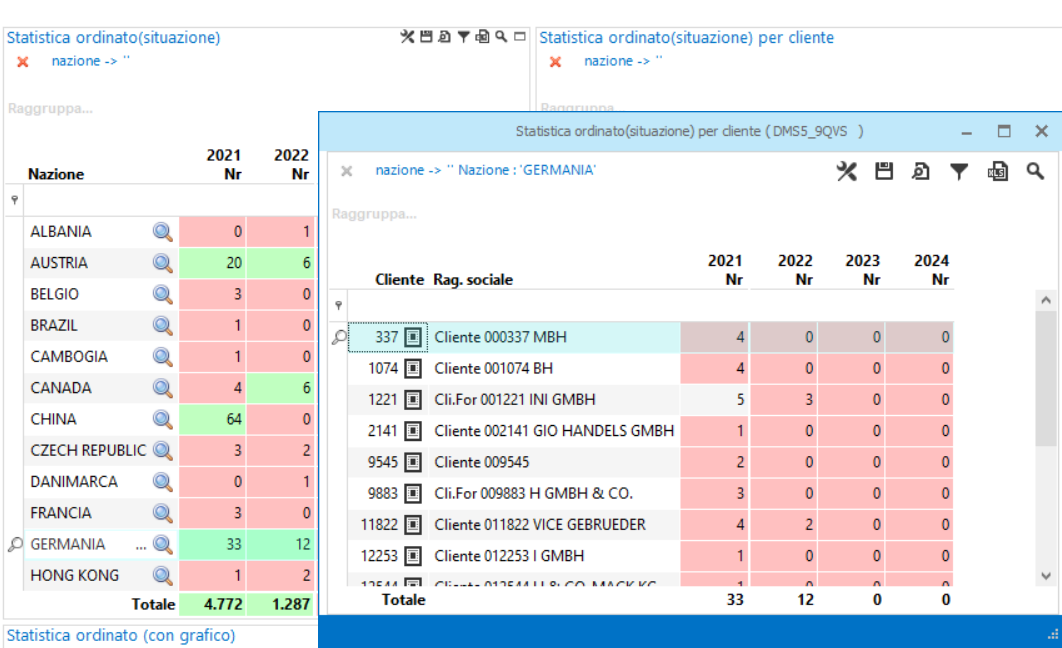
\includegraphics[width=\linewidth]{quickvision/apertura tabella cliente.png}
        \caption{Apertura di "Statistica ordinato per cliente" da "Statistica ordinato"}
    \end{minipage}
    \hfill
    \begin{minipage}{0.45\textwidth}
        \centering
        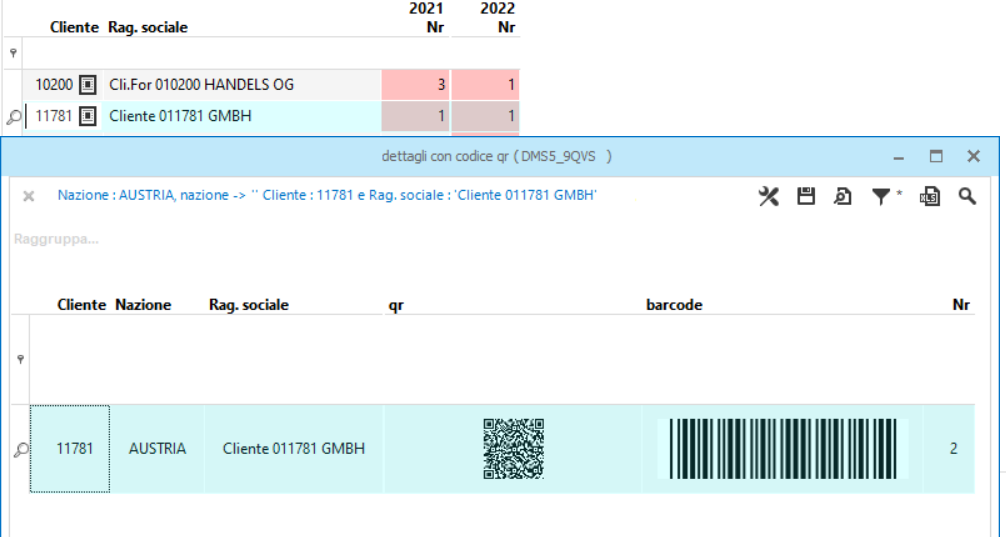
\includegraphics[width=\linewidth]{quickvision/apertura tabella qr.png}
        \caption{Apertura di "Dettagli con codice qr" per cliente da "Statistica ordinato per cliente"}
    \end{minipage}
\end{figure}


In quickvision una tabella e un grafico sono lo stesso elemento (denominato "situazione") che differisce per come vengono presentati i dati e per le proprietà del grafico stesso.
I grafici cambiano dinamicamente se la tabella a cui sono associati subisce un interazione.
Nel progetto alla selezione di una riga il grafico mostrerà solo le statistiche riguardanti quella riga invece dell'intera tabella.

\begin{figure}[h]
    \centering
    \begin{minipage}{0.45\textwidth}
        \centering
        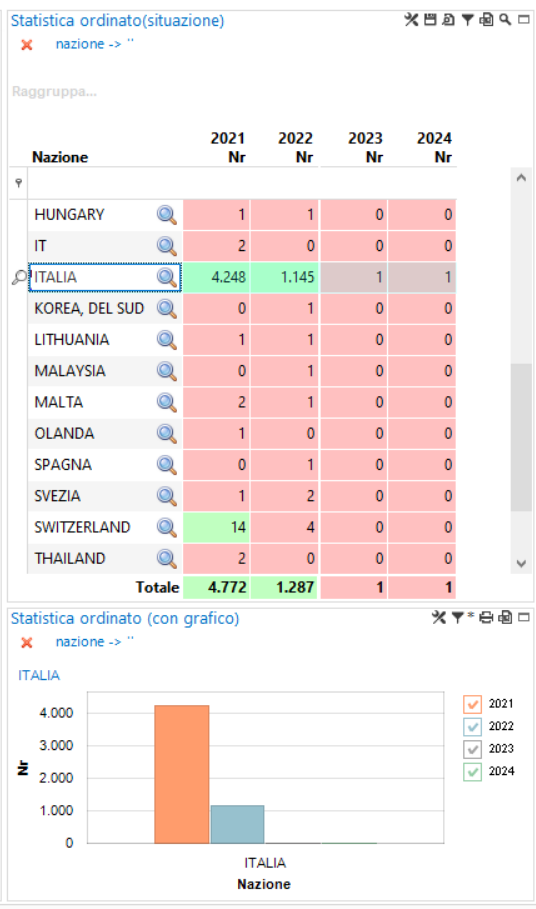
\includegraphics[ width=0.6\linewidth]{quickvision/tabella cliente.png}
        \caption{Statistica ordinato con tabella dinamica}
    \end{minipage}
    \hfill
    \begin{minipage}{0.45\textwidth}
        \centering
        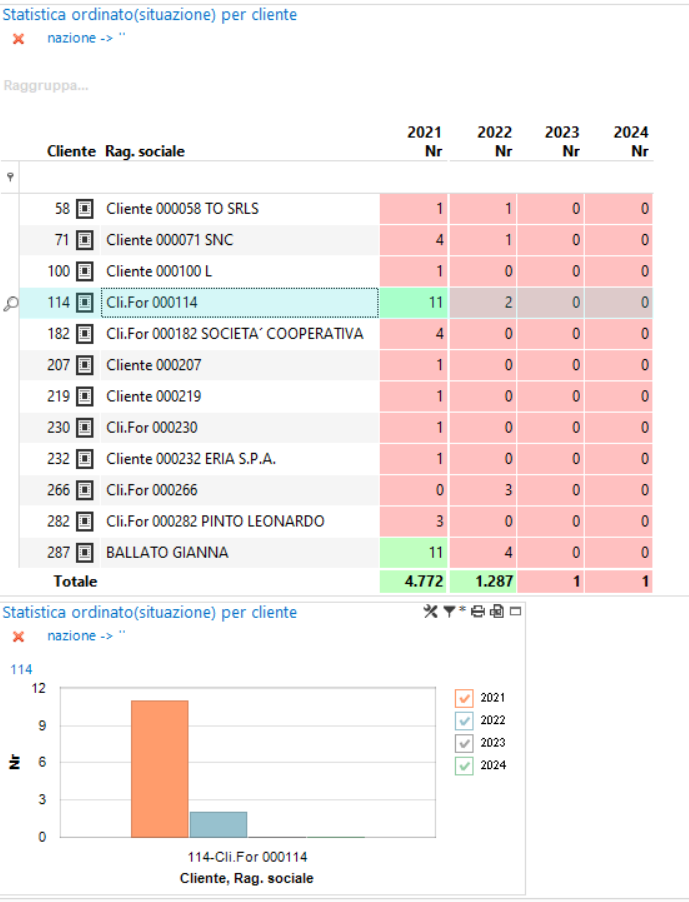
\includegraphics[width=0.75\linewidth]{quickvision/tabella nazione.png}
        \caption{Statistica ordinato per clienti con tabella dinamica}
    \end{minipage}
\end{figure}


\begin{figure}[H]
    \centering
    \begin{minipage}{0.45\textwidth}
        \centering
        \includegraphics[ width=0.8\linewidth, trim=13cm 16cm 25cm 3cm, clip]{quickvision/tabella nazioni proprietà.png}
        \caption{struttura tabella Statistica ordinato}
    \end{minipage}
    \hfill
    \begin{minipage}{0.45\textwidth}
        \centering
        \includegraphics[width=0.8\linewidth, trim=13cm 16cm 25cm 4cm, clip]{quickvision/tabella clienti proprietà.png}
        \caption{struttura tabella Statistica ordinato per clienti}
    \end{minipage}
\end{figure}


\subsection{Creazione di uno schema}

\begin{wrapfigure}{r}{0.5\textwidth}
    \centering
    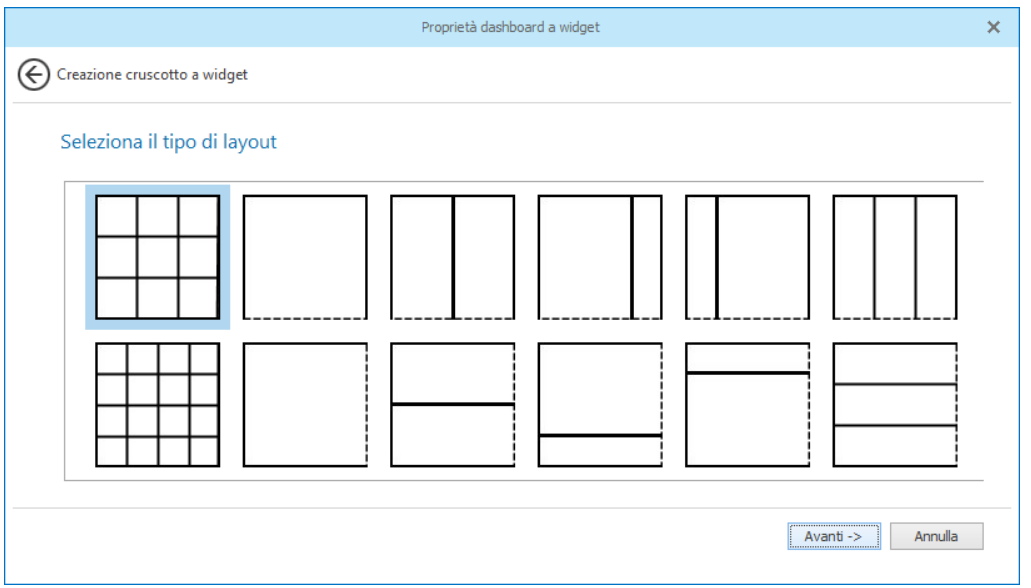
\includegraphics[width=0.5\textwidth]{quickvision/configurazione schema.png}
    \caption{Selezione del layout dello schema}
\end{wrapfigure}

Uno schema è un insieme di elementi mostrati su un unica pagina al fine di creare un pannello di controllo.
Gli elementi inseribili in uno schema sono grafici e tabelle realizzati precedentemente, pulsanti link, pulsanti filtro e loghi. Un elemento può essere aggiunto tramite l'apposito menu.
Tramite uno schema è possibile quindi creare pannelli di controllo su misura.
In ambito lavorativo per esempio possiamo creare diversi schemi per diversi uffici sotto la stessa sorgente dati mostrando solo i dati di interesse di quell'ufficio.

A differenza delle tabelle, uno schema viene creato tramite una procedura guidata esterna al pannello di configurazione del progetto.
Lo schema comparirà e sarà modificabile anche dal pannello di configurazione del progetto, procedura consigliata solo agli sviluppatori esperti con l'ambiente quickvision.
\begin{figure}[H]
    \centering
    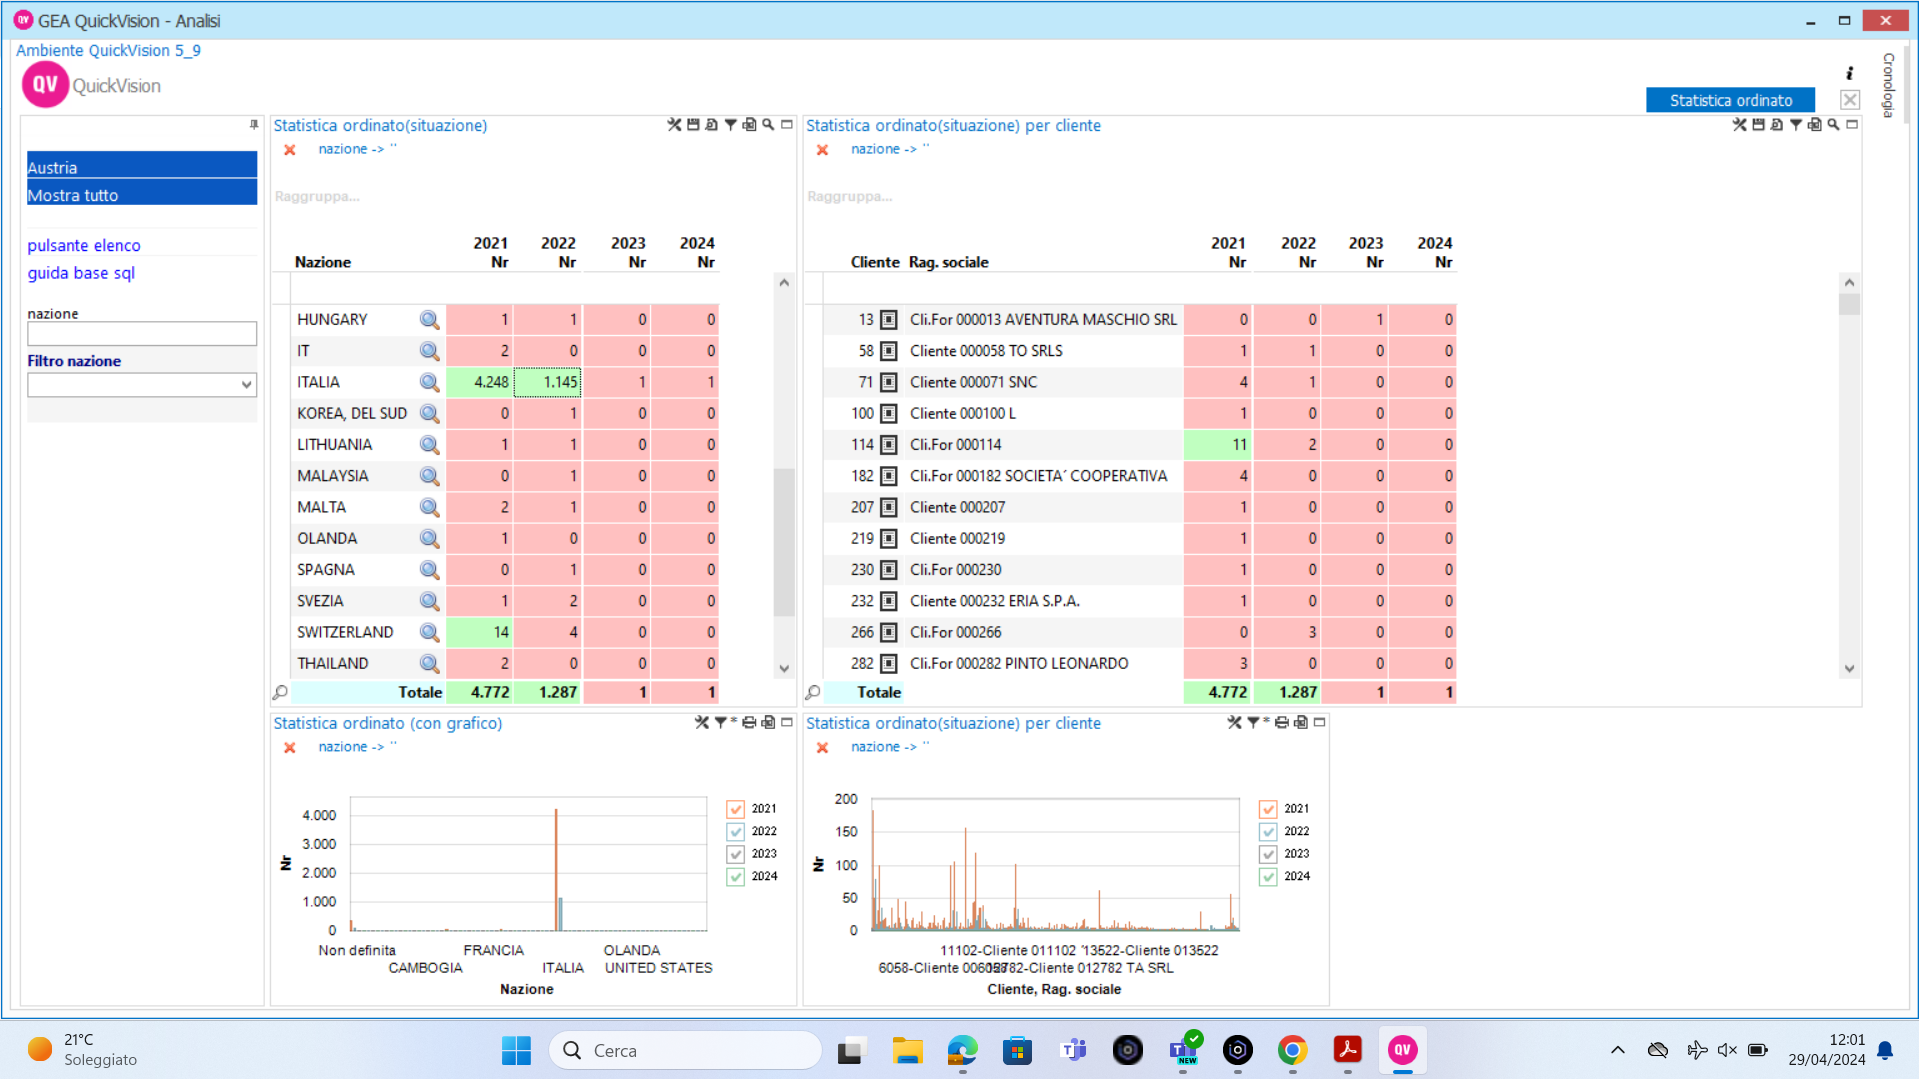
\includegraphics[width=0.7\textwidth]{quickvision/schema.png}
    \caption{Schema del progetto}
\end{figure}

\subsection{Pulsanti}


Con l'utilizzo di uno schema posso configurare dei filtri globali tramite l'inserimento di un pulsante filtro. 
Questi filtri avranno effetto su tutte le situazioni presenti all'interno dello schema stesso.
Il progetto possiede un filtro globale per nazione rappresentato in 3 modi diversi:


\begin{enumerate}
    \item pulsante tradizionale, il filtro viene rappresentato da un singolo pulsante che applica uno specifico filtro assegnato.
    \item casella di testo, il filtro viene applicato in base al contenuto della casella di testo. 
    \item listbox a selezione multipla, mostra una lista di tutti i possibili valori che il filtro può assumere. Piu di un elemento può essere selezionato per la visualizzazione.
\end{enumerate}

I pulsanti possono anche contenere collegamenti ipertestuali. 
Nel progetto è presente un pulsante per la visualizzazione di un file pdf di esempio: la guida a sql fornita dall'azienda.

\begin{figure}[H]
    \centering
    \begin{minipage}{0.45\textwidth}
        \centering
        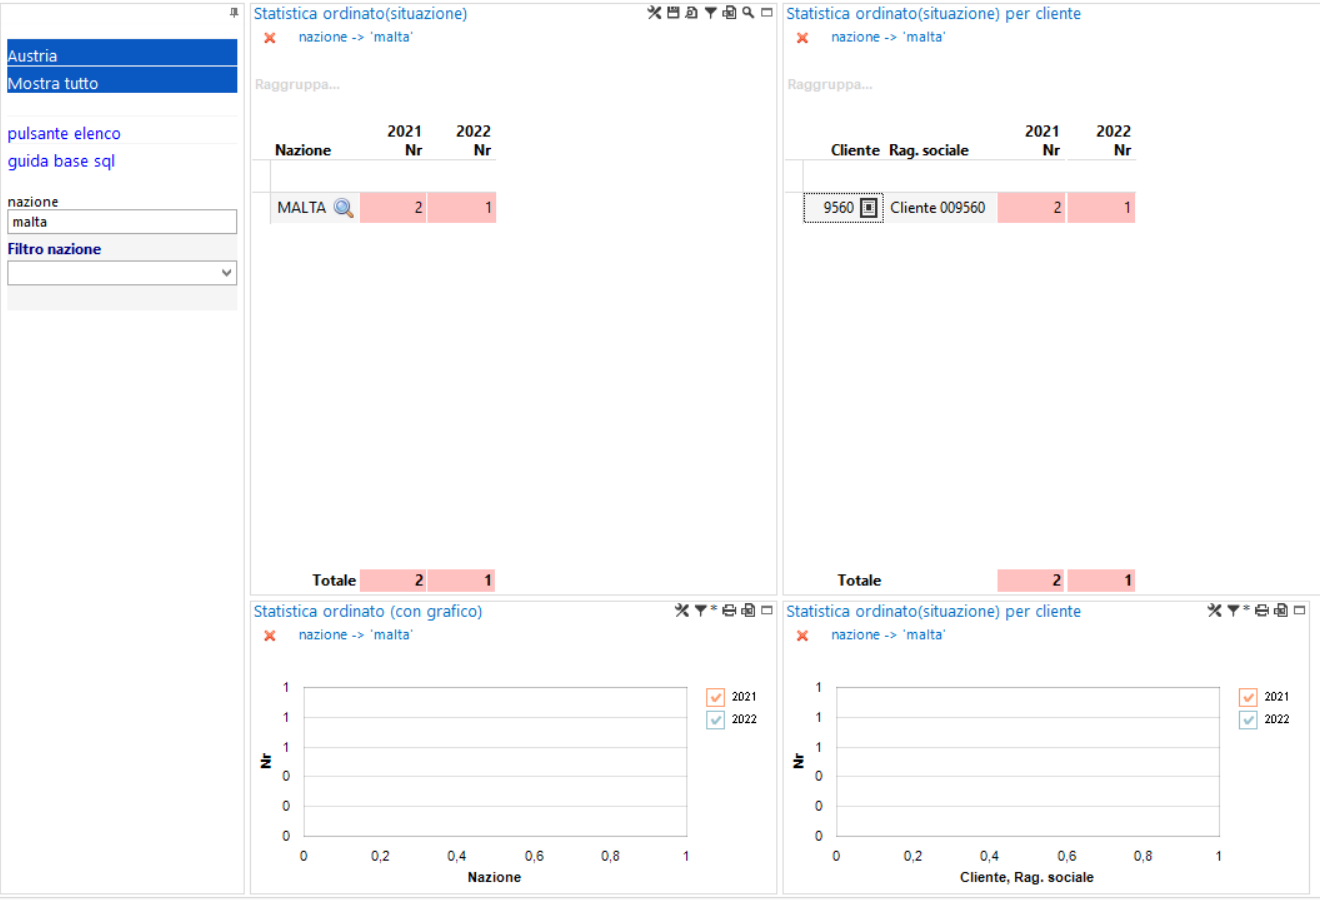
\includegraphics[width=\linewidth, trim=0cm 0cm 15cm 0cm, clip]{quickvision/filtro.png}
        \caption{Filtro applicato casella di testo}
    \end{minipage}
    \hfill
    \begin{minipage}{0.45\textwidth}
        \centering
        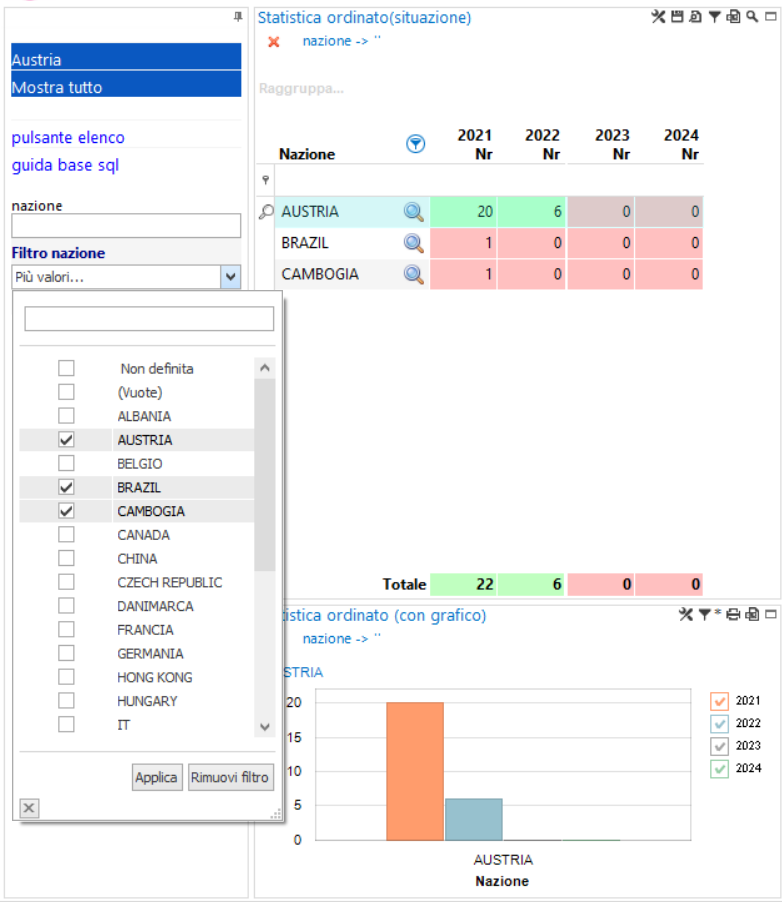
\includegraphics[width=\linewidth]{quickvision/filtro list.png}
        \caption{Filtro applicato tramite listbox}
    \end{minipage}
\end{figure}


\subsection{Conclusione}
Il progetto concluso è un esempio di pannello di controllo per il monitoraggio e l'analisi degli ordini dei clienti.
Questo pannello è accompagnato da opportuni grafici, filtri e tabelle interattive.
La configurazione delle tabelle e dello schema è salvata sottoforma di file xml.
\begin{figure}[H]
    \centering
    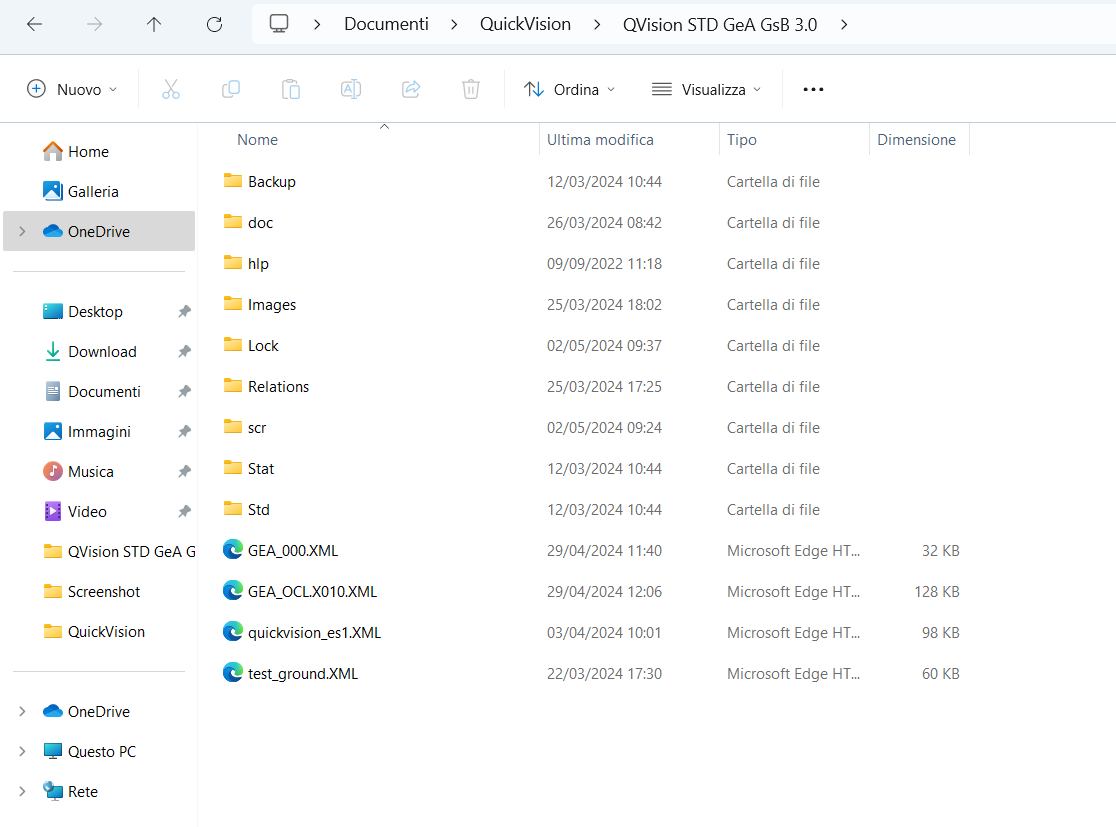
\includegraphics[width=0.5\textwidth]{quickvision/cartella progetto.png}
    \caption{Cartella dei progetti}
\end{figure}

%%------------------------------------------------------------------------------------------------------------------------------------------------------------------------------------------------------


\chapter{Programma finale, richieste ferie e permessi via app}
\section{Obbiettivo}
L'obbiettivo del programma è di aggiornare l'attuale sistema di richiesta delle assenze, presente nel gestionale dell'azienda, con uno in grado di funzionare su sistemi mobili.

\subsection{Richieste}
\begin{enumerate}
    \item L'entry form deve avere una struttura come mostrato nell'immagine.
    \item Per l'inserimento di un nuovo elemento deve essere richiesto prima la causale e poi l'intervallo di tempo che si adatterà in base alla causale richiesta.
    Per le ferie si specifica un intervallo di date mentre per i permessi un intervallo in ore.
    \item La lista delle causali si ottiene tramite una query già fornita.
    \item l'inserimento dei dettagli dell'assenza deve avvenire in "steps". Certi campi di input vengono rivelati a ogni step per guidare l'utente nell'inserimento.
    \item I pulsanti "Da autorizzare" e "Autorizzate" devono contenere un conteggio degli elementi al loro interno nel testo del bottone.
    \item Le liste di assenze di "Da autorizzare" e "Autorizzare" devono utilizzare una specifica query sql fornita per il recupero delle informazioni. 
    \item Ogni riga delle liste deve contenere un bottone per visualizzarne (se autorizzata) o modificarne (se da autorizzare) i dettagli relativi alla durata dell'assenza.
    \item Il layout dell'applicazione deve essere di facile utilizzo per utenti da mobile.
\end{enumerate}

\section{Progettazione}%schemi di layout fatti con il tutor, schemi di funzionamento, activity diagram, state diagram

\subsection{Diagramma dei casi d'uso}
Per rappresentare le richieste viene implementato un diagramma dei casi d'uso.

\begin{figure}[H]
    \centering
    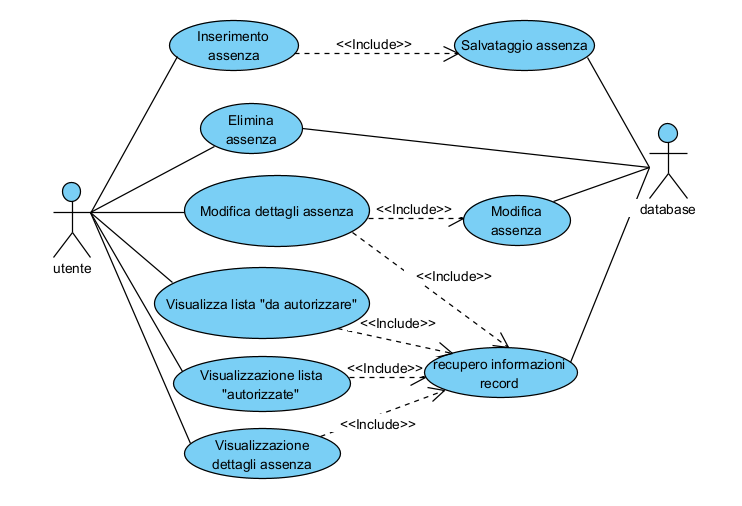
\includegraphics[width=0.6\textwidth]{diagrammi/caso d'uso finale.png}
    \caption{Diagramma dei casi d'uso}
\end{figure}

\subsection{Diagramma degli stati}
Poiché il programma interagisce con l'utente aprendo e chiudendo le diverse schermate, possiamo rappresentare il funzionamento del progetto tramite uno state diagram.

\begin{figure}[H]
    \centering
    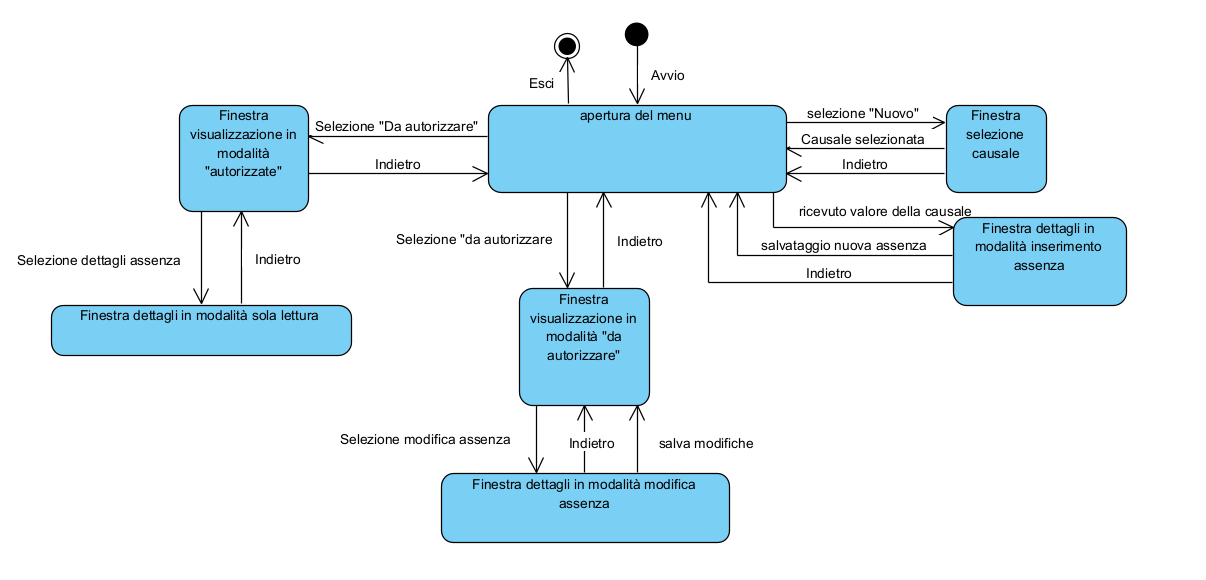
\includegraphics[width=0.8\textwidth]{diagrammi/state progetto finale.png}
    \caption{Diagramma degli stati}
\end{figure}

\newpage
\subsection{Flusso del programma}
Come visto per il primo progetto, il flusso dei programmi rpgle è prestabilito dall'azienda.
Possono essere apportate modifiche, ma non può essere modificato il flusso del programma.
Ogni nuova funzione deve essere richiamata all'interno dell'opportuna funzione del flusso.
Per lo schema del flusso si fa riferimento alla figura 5.3.


\section{GSA080}
\subsection{Funzionalità}
GSA080 è il programma che si occupa della gestione del menu principale. Da qui possiamo accedere a tutte le funzionalità principali del progetto tramite i 3 bottoni presenti.



\begin{itemize}
    \item \textbf{Nuovo} invoca l'interfaccia di GSA082 che si occupa della selezione della motivazione di assenza. 
    Se questa viene selezionata, GSA082 ritorna il valore della causale. 
    Quando viene ricevuto un valore da GSA082, GSA080 apre l'interfaccia di GSA084 con il valore ricevuto sottoforma di parametro in input.
    GSA084 si occuperà quindi dell'inserimento dei dettagli. 
        
    \item \textbf{Da approvare} apre l'interfaccia di GSA081 che elenca tutte le richieste di assenza non ancora approvate dall'azienda. Il pulsante mostrerà nel suo testo il numero di elementi da approvare.
    
    \item \textbf{Approvate} apre anchesso l'interfaccia di GSA081 ma verranno visualizzate solo le assenze già approvate dall'azienda. Il pulsante mostrerà nel suo testo il numero di elementi approvati.
\end{itemize}

\begin{figure}[h]
    \centering
    \begin{minipage}{0.45\textwidth}
        \centering
        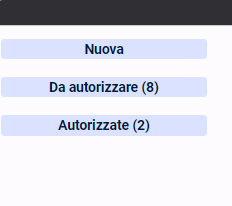
\includegraphics[width=\linewidth]{screenshot/Interfaccia_gsa080.png}
        \caption{schermata GSA080}
    \end{minipage}
    \hfill
    \begin{minipage}{0.45\textwidth}
        \centering
        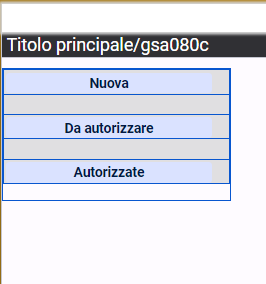
\includegraphics[width=\linewidth]{screenshot/Struttura_gsa080.png}
        \caption{struttura della schermata GSA080}
    \end{minipage}
\end{figure}


\subsection{Funzioni principali}
Lodhf0 è la funzione che gestisce il caricamento delle informazioni relative agli elementi di hf0.
In questo programma si occupa del conteggio di assenze da approvare e approvate al fine di aggiornare i valori mostrati. Se non sono presenti assenze, il bottone relativo viene disattivato.


\begin{lstlisting}[language=RPG, caption=Codice RPG di Lodhf0, label=lst:rpgHF0BTNNEW]
    //ricava numero assenze da autorizzare
    exec sql select count(distinct gsaidn)
            into :QvlCount
            from gstgas00v join grtang00f on grtidn=gsagrtidn
            where gsaaznidn=1
                and gasdteass>=:QvgDteCmp
                and gsarsuidn=:QprIdnRsu
                and GrtGstPrm = '1'
                and gsasttaur='1';

    setatr(QvgFrm:'hf0btndau':'xdsc':'Da autorizzare ('+%char(QvlCount)+')');

    if QvlCount=0;
        setatr(QvgFrm:'hf0btndau':'disabled':'disabled');
    endif;
\end{lstlisting}

Il codice per le assenze da autorizzare è analogo con l'unica differenza che gsasttaur='5'.


Cnthf0 si riferisce al codice che gestisce cambiamenti all'interno di hf0.
Nello specifico questa funzione gestisce i cambiamenti avvenuti negli elementi di hf0 ossia i 3 bottoni del menu.

Il bottone HF0BTNNEW è il bottone che apre le interfacce volte all'inserimento di una nuova assenza.
\begin{lstlisting}[language=RPG, caption=Codice RPG del bottone HF0BTNNEW, label=lst:rpgHF0BTNNEW]
    // Nuova
    if QdgFrm.HF0BTNNEW='*on';
        // selezione causale
        clear QvgPrmInp ;
        QvgFrmCnl='GSA082C';
        FrmCnl(QvgPrmInp);
        QvlIdnGrt= gpn(QvgPrmInp:'qpridngrt');  //valore ritornato da gsa082c

        // inserimento richiesta
        if QvlIdnGrt <> 0;
        clear QvgPrmInp ;
            QvgPrmInp = ap(QvgPrmInp:'qpridnrsu':%char(QprIdnRsu):' ');
            QvgPrmInp = ap(QvgPrmInp:'qpridngrt':%char(QvlIdnGrt):' ');
            QvgPrmInp = ap(QvgPrmInp:'qpridngsa':'0':' ');
            QvgFrmCnl='GSA084C';
            FrmCnl(QvgPrmInp);
            QvgFlgRcr=gp(QvgPrmInp:'qprflgupd');
        endif;
    endif;
\end{lstlisting}

\section{GSA081}
\subsection{Funzionalità}
GSA081 si occupa del mostrare a schermo una lista di assenze. Viene utilizzato per mostrare sia le assenze da autorizzare che quelle autorizzate.
In base ai parametri di input il programma decide che assenze visualizzare e che funzioni rendere disponibili all'utente.

Nel caso della lista assenze da autorizzare sarà disponibile un bottone per apporre modifiche ai dati e uno per la cancellazione della richiesta.

Nel caso della lista assenze autorizzate il pulsante di modifica svolgerà la funzione di pulsante di visualizzazione dei dettagli mentre il pulsande di cancellazione viene nascosto.

\begin{figure}[h]
    \centering
    \begin{minipage}{0.3\textwidth}
        \centering
        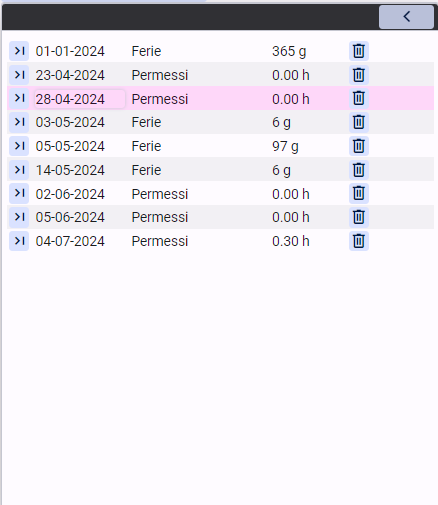
\includegraphics[width=\linewidth]{screenshot/Interfaccia_gsa081_DAU.png}
        \caption{schermata GSA081 per assenze da autorizzare}
    \end{minipage}
    \hfill
    \begin{minipage}{0.3\textwidth}
        \centering
        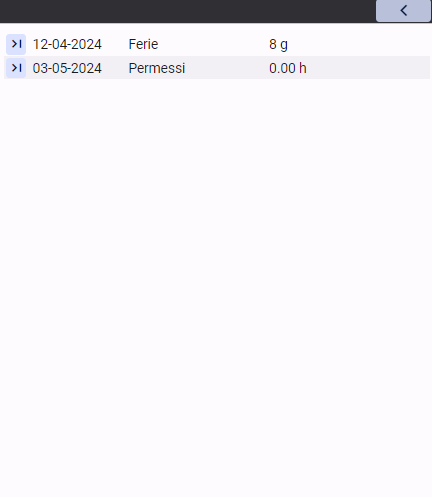
\includegraphics[width=\linewidth]{screenshot/Interfaccia_gsa081_AUT.png}
        \caption{schermata GSA081 per assenze autorizzate}
    \end{minipage}
    \hfill
    \begin{minipage}{0.3\textwidth}
        \centering
        \includegraphics[width=\linewidth]{screenshot/Struttura_gsa081.png}
        \caption{struttura della schermata GSA081}
    \end{minipage}
\end{figure}

\break
\subsection{Funzioni principali}



Lodhf0 si occupa del recupero dei dati della lista di assenze tramite un interrogazione SQL. 
QprSttAss contiene il valore che differenzia le assenze autorizzate da quelle da autorizzare.
L'interrogazione sql è stata fornita dall'azienda e, come da loro richiesto, non è stata alterata.

\begin{lstlisting}[language=RPG, caption=Codice RPG per la costruzione dell'interrogazione SQL]
    QvlStrSql = 'select gsaidn, tpo.dbqdsc, '' '', +
                    min(gasdteass), max(gasdteass), +
                    gsasttaut, gsasttaur, sttaut.dbqdsc, +
                    coalesce(sttaur.dbqdsc, ''''), +
                    sum(case w hen gastpoass=''1'' then 1 else 0 end), +
                    sum(case w hen gastpoass=''0'' then gasmmass else 0 end) +
                from gstgas00v +
                join grtang00f on gsagrtidn=grtidn +
                join dbqang00f tpo on tpo.dbqtblnme=''GRTANG00F'' +
                    and tpo.dbqclnnme=''GRTTPO'' +
                    and tpo.dbqvle=grttpo +
                join dbqang00f sttaut on sttaut.dbqtblnme=''GSTASS00F'' +
                    and sttaut.dbqclnnme=''GSASTTAUT'' +
                    and sttaut.dbqvle=gsasttaut +
                left join dbqang00f sttaur on sttaur.dbqtblnme=''GSTASS00F'' +
                    and sttaur.dbqclnnme=''GSASTTAUR'' +
                    and sttaur.dbqvle=gsasttaur +
                :where and gsaaznidn=' +%char(QdgPnv.idnazn)+ ' +
                    and gsarsuidn=' +%char(QvgRsuIdn)+ ' +
                    and gasdteass>' +%char(UDATE)+ ' +
                    and gststtaur=''5 '' +
                    and GrtGstPrm = ''1'' +
                group by gsaidn, tpo.dbqdsc, +
                    gsasttaut, gsasttaur, sttaut.dbqdsc, +
                    sttaur.dbqdsc +
                :order 4 +
                fetch first 10000 row s only +
                for read only +
\end{lstlisting}

\break

Wrthg0() si occupa delle modifiche da apportare alla lista hg0.
Le modifiche applicate includono il popolamento della lista, lo scorrimento delle pagine della lista (qualora venissero superate le righe massime per pagina) 
e l'occultamento del bottone di cancellazione per la lista di assenze autorizzate.
La durata dell'assenza viene mostrata sottoforma di giorni invece di ore nel caso di ferie.

\begin{lstlisting}[language=RPG, caption=Codice RPG di occultamento del bottone elimina(h50btndlt), label=lst:rpglodhf0gsa081]
    //se autorizzato nascondi bottone elimina
    if QprSttAss = '5';
        addatr(QvgFrm:'h50btndlt':'class':'hidden');
    endif; 
\end{lstlisting}


Cnthg0() controlla il cambiamento dello stato della lista e dei suoi elementi.
In GSA081 controlla i pulsanti di scorrimento delle pagine, il pulsante di modifica/visualizzazione dettagli e il pulsante di cancellazione.
\begin{lstlisting}[language=RPG, caption=Codice RPG di controllo dei pulsanti]
// richiama dettaglio assenza
if QdgFrm.H50BTNSLZ='*on';
    clear QvgPrmInp;
    //parametri in input all'interfaccia GSA084 (chiave del record corrispondente)
    QvgPrmInp=ap(QvgPrmInp:'qpridngsa':Qdgh50(QvlCount).h50idn:' ');
    QvgFrmCnl='GSA084C'; //apertura dell'interfaccia GSA084
    FrmCnl(QvgPrmInp);
    QvgFlgRcr=gp(QvgPrmInp:'qprflgupd');
endif;

if QdgFrm.H50BTNDLT ='*on';
    //operazione di cancellazione del record corrispondente
    QdgRtc=GsaDlt(%int(Qdgh50(QvlCount).h50idn):'msg'); 
    if QdgRtc.exc='true';
        QvgFlgRcr='si';
    return;
    endif;
endif;
\end{lstlisting}
\break




\section{GSA082}

\subsection{Funzionalità}
GSA082 è l'interfaccia che si occupa di mostrare una lista di causali possibili da inserire nella richiesta di assenza.
\\Le causali vengono prelevate dalla tabella "tblaut00f" del database.
\\Ogni riga della lista contiene una lable per contenere il nome della causale e un bottone che ritornerà il valore di quella causale a GSA080.

\begin{figure}[h]
    \centering
    \begin{minipage}{0.45\textwidth}
        \centering
        \includegraphics[width=\linewidth]{screenshot/Interfaccia_gsa082.png}
        \caption{schermata GSA080}
    \end{minipage}
    \hfill
    \begin{minipage}{0.45\textwidth}
        \centering
        \includegraphics[width=\linewidth]{screenshot/Struttura_gsa082.png}
        \caption{struttura della schermata GSA080}
    \end{minipage}
\end{figure}

\subsection{Funzioni principali}
Lodhg0 si occupa della costruzione ed esecuzione della richiesta in sql per ricavare tutte le possibili causali delle assenze.
\begin{lstlisting}[language=RPG, caption=Codice RPG di controllo dei pulsanti]
 QvlSqlStr = 'select +
                    grtidn, +
                    grtdsc +
                from GRTANG00F +
            :where +
                and grtgstass=''1'' +
                and grttpo in (''3'', ''4'') +
                and grtgstprm = ''1'' +
            group by grtdsc,grtidn +
            :order grtdsc +
                fetch first :elem rows only +
                for read only';

// Valorizza numero massimo elementi
QvlSqlStr = %scanrpl(':elem':%char(QvlElm):QvlSqlStr);
// Build where condition
QvlSqlStr = %scanrpl(':where':
                    BldWhr(QvgFrm:getatr(QvgFrm:'h20':'xwhrstr')):
                    QvlSqlStr);
// Build order condition
QvlSqlStr = %scanrpl(':order':
                    BldOrd(QvgFrm:getatr(QvgFrm:'h20':'xordstr')):
                    QvlSqlStr);
\end{lstlisting}

Cnthg0 controlla i bottoni di scorrimento della pagina e il bottone di selezione della causale.
In base al bottone premuto, il programma restituisce il relativo identificativo (conservato in un campo nascosto h50idn nella tabella).
Questo valore viene poi salvato in QprStr, stringa contenente i parametri da restituire al termine del programma.
\begin{lstlisting}[language=RPG, caption=Codice RPG di controllo dei pulsanti]
// seleziona giustificativo
    if QdgFrm.H50BTNSLZ='*on';
        QvgIdnGrt=%int(g(QvgFrm:'h50idn':QvlCount));  //ricavo la chiave salvata nella riga selezionata
        FrmEnd();
        return;
    endif;

    //------------al termine del programma----------
    // Valorizza Parametri Output
    QprStr = ap(QprStr:'qpridngrt':%char(QvgIdnGrt):'');
\end{lstlisting}
\break

\section{GSA083}
GSA083 si occupa della visualizzazione e/o della modifica dei dettagli relativi alle assenze.
Questo programma è stato completamente sostituito con GSA084 in seguito a una modifica richiesta.


\section{GSA084}
\subsection{Funzionalità}
GSA084 è l'interfaccia che si occupa dell'inserimento e della modifica delle assenze.

Per distinguere un inserimento da una modifica, il programma controlla il valore in input di QvgIdnGsa, ossia la variabile contenente la chiave di un record della tabella delle assenze.
Se è uguale a 0 vuol dire che il valore non è presente nel nostro database e quindi si procede con un inserimento.
Se è diverso da 0 questo valore viene usato per recuperare i dati dell'assenza.

Se sto inserendo una nuova assenza, il programma mostra a schermo solo i campi da compilare di mio interesse.

Tra i parametri in input viene passato il record della causale dell'assenza selezionato precedentemente. Da questo record estrapoliamo il tipo e confrontiamo il suo valore.
Se è uguale a 3 sono in presenza di ferie perciò nasconderò i campi relativi all'inserimento delle ore poiché le ferie devono durare almeno un giorno.
Se è uguale a 4 sono invece in presenza di permessi quindi nascondo la data di termine mantenendo gli input degli orari. Un permesso infatti è previsto occupi solo parte della stessa giornata.


Per distinguere una modifica da una visualizzazione il programma controlla il valore del parametro sttaur, parametro che contiene lo stato della autorizzazione.
Se è 1, quindi assenza da autorizzare, inserisco i valori correnti nei campi di input per aggevolare la modifica.
Se è 5, perciò assenza autorizzata, i campi di input vengono popolati con in valori dell'assenza ma impostati in sola lettura cosi da non poter apportare modifiche.

Prima che l'inserimento o la modifica vada a buon fine vengono messi in atto diversi controlli sulla correttezza dei dati inseriti

\begin{figure}[h]
    \centering
    \begin{minipage}{0.3\textwidth}
        \centering
        \includegraphics[width=\linewidth]{screenshot/Interfaccia_gsa084_ferie.png}
        \caption{schermata GSA084 per dettagli delle ferie}
    \end{minipage}
    \hfill
    \begin{minipage}{0.3\textwidth}
        \centering
        \includegraphics[width=\linewidth]{screenshot/Interfaccia_gsa084_AUT.png}
        \caption{schermata GSA084 per dettagli dei permessi}
    \end{minipage}
    \hfill
    \begin{minipage}{0.3\textwidth}
        \centering
        \includegraphics[width=\linewidth]{screenshot/Struttura_gsa084.png}
        \caption{struttura della schermata GSA084}
    \end{minipage}
\end{figure}

\subsection{Funzioni principali}
Lodhf0 si occupa del abilitare o nascondere gli elementi dell'interfaccia in base alla presenza di un assenza per permesso o per ferie.
Nel caso l'interfaccia sia aperta con richiesta di inserimento verranno eseguiti 2 step:
\begin{enumerate}
    \item Viene richiesto di inserire la data dell'assenza. Questa data sarà il primo giorno di un intervallo di date oppure il giorno stesso di un assenza di poche ore. Il pulsante avanti viene rinominato salva per lo step successivo. I campi compilati vengono resi in sola lettura.
    \item in base alla causale vengono mostrate 2 situazioni differenti:
    \begin{enumerate}
            \item la causale descrive un periodo di ferie. In questo caso viene richiesta una seconda data per definire il termine dell'assenza nascondendo i campi superflui.
            \item la causale descrive un permesso di assenza. In questo caso viene richiesto l'orario di inizio e di fine assenza nascondendo i campi superflui. 
    \end{enumerate}
\end{enumerate}

Nel caso di modifica di un'assenza non saranno eseguiti step. I campi idonei, ossia quelli pertinenti al tipo di assenza da modificare, saranno tutti modificabili da subito e vengono popolati con i dati correntemente memorizzati.

Infine nel caso di visualizazione delle assenze si procede come per le modifiche. Tutti i campi idonei sono mostrati e popolati ma impostati in sola lettura. Inoltre il pulsante di salvataggio viene nascosto lasciando solo il pulsante indietro per tornare alla schermata che ha richiamato GSA084.
\\
\\Cnthf0 gestisce il controllo dei pulsanti e degli errori.
\\Riguardo la gestione degli errori il sistema prevede i seguenti controlli:
\\
\\Per le date avviene un controllo tramite la funzione ChkDte() che verifica i seguenti casi:
\begin{enumerate}
    \item Mancato inserimento del giorno
    \item Mancato inserimento del mese
    \item Mancato inserimento dell'anno
    \item Giorno non contenuto nel mese
    \item Anno bisestile
    \item La data supera la data di chiusura del consuntivo
    \item La data supera l'ultimo giorno del calendario aziendale
\end{enumerate}
Per le ore inserite il controllo avviene tramite la funzione ChkOra() che verifica i seguenti casi:
\begin{enumerate}
    \item Mancato inserimento dell'ora di inizio
    \item Mancato inserimento dell'ora di fine
    \item Ora di fine minore dell'ora di inzio
\end{enumerate}

\begin{figure}[h]
    \centering
    \includegraphics[width=0.35\linewidth]{screenshot/Interfaccia_gsa084_errore.png}
    \caption{Errore di mancato inserimento evidenziato in rosso}
\end{figure}

\section{Adattamento per mobile}
Affinché l'applicazione sia adatta per l'uso da mobile è necessario riadattare le schermate e ridimensionare i pulsanti.
Per mantenere le correnti proporzioni per l'uso da desktop, vengono create delle copie dei file.
Questi file si chiameranno GSAxxxc\_smartphone.xml.
Il suffisso \_smartphone è una parola chiave riconosciuta automaticamente da unigea. Se il programma viene eseguito da mobile, unigea automaticamente userà la struttura mobile mantnendo lo stesso file rpgle per la logica di funzionamento.
\begin{figure}[h]
    \centering
    \includegraphics[width=0.6\linewidth]{screenshot/Lista_gsb120.png}
    \caption{Lista dei file xml delle schermate di GSB120 per desktop e mobile}
\end{figure}
\newpage
\begin{figure}[H]
    \centering
    \begin{minipage}{0.25\textwidth}
        \centering
        \includegraphics[width=\linewidth]{screenshot/mobile GSA080.png}
        \caption{schermata principale per dispositivi mobili}
    \end{minipage}
    \hfill
    \begin{minipage}{0.25\textwidth}
        \centering
        \includegraphics[width=\linewidth]{screenshot/Mobile GSA082.png}
        \caption{schermata selezione causale per dispositivi mobili}
    \end{minipage}
    \hfill
    \begin{minipage}{0.25\textwidth}
        \centering
        \includegraphics[width=\linewidth]{screenshot/Mobile GSA084 step1.png}
        \caption{schermata di inserimento assenza per dispositivi mobili}
    \end{minipage}
\end{figure}

\begin{figure}[H]
    \centering
    \begin{minipage}{0.25\textwidth}
        \centering
        \includegraphics[width=\linewidth]{screenshot/Mobile GSA084 Ferie.png}
        \caption{schermata di inserimento ferie per dispositivi mobili}
    \end{minipage}
    \hfill
    \begin{minipage}{0.25\textwidth}
        \centering
        \includegraphics[width=\linewidth]{screenshot/Mobile GSA084 Permesso.png}
        \caption{schermata di inserimento permesso per dispositivi mobili}
    \end{minipage}
    \hfill
    \begin{minipage}{0.25\textwidth}
        \centering
        \includegraphics[width=\linewidth]{screenshot/Mobile GSA081 da approvare.png}
        \caption{schermata di visualizzazione richieste per dispositivi mobili}
    \end{minipage}
\end{figure}

%% Fine dei capitoli normali, inizio dei capitoli-appendice (opzionali)
\appendix

%\part{Appendici}

\chapter{Protocollo GSB}

Per poter correttamente utilizzare le risorse aziendali e permettere una successiva modifica del programma da parte dell'azienda, è necessario conoscere il protocollo GSB ossia gli standard di denominazione dell'azienda.
\section{Nomenclatura archivi}
La nomenclatura degli archivi segue lo schema xxxxxx99z:

xxxxxx identifica il nome del record.

99 è un numero progressivo.

z definisce il tipo di file:
\begin{itemize}
    \item F fisico
    \item I indice
    \item A indice automatico
    \item V view
\end{itemize}

Esempio: BPNANG00F Tabella business partners - anagrafica.

\section{Nomenclatura programmi}
Per i programmi si segue lo schema xxx99z

\begin{itemize}
    \item xxx è il nome dell'applicazione.

    \item 999 è un numero progressivo.
    \begin{itemize}
        \item da 000 a 899 - Gestione, visualizzazione, stampe e utilità
        \item da 900 a 999 - Pannelli innestati
    \end{itemize}

    \item z deginisce il tipo di file.
    \begin{itemize}
        \item C controller
        \item R controller tampe
        \item I controller pannelli innestati
    \end{itemize}
\end{itemize}
\section{Nomenclatura campi}

I nomi delle variabili usate nella definizione degli archivi possono essere lunghi al massimo 10 caratteri e
devono rispettare la seguente struttura:
XxxYyy(Zzzz)

\begin{itemize}
    \item Xxx identifica il prefisso dell'archivio oppure il suo uso

    \item Yyy definisce il tipo di campo

    \item Zzzz definisce l'identificativo della variabile. Questo è opzionale.
    \begin{itemize}
        \item La serie di caratteri che identifica la variabile deve essere lunga da un minimo di 3 ad un massimo di 4.
        \item Eliminare le vocali, tranne nel caso in cui la parola da descrivere inizi con una vocale.
        \item Eliminare le doppie, tranne nel caso in la contrazione porti ad una definizione non significativa.
        \item Nel caso in cui l’entità da descrivere sia composta da più parole contrarre in funzione della parola più
        significativa.
    \end{itemize}
\end{itemize}


\section{Nomenclatura record}
I nomi delle variabili usate nella definizione dei record devono essere lunghi 6 caratteri e devono rispettare la
seguente struttura:
QxxYyy
\begin{itemize}
    \item Q è fisso e sempre presente all'inizio della variabile

    \item xx definisce l'uso
    \begin{itemize}
        \item dg=globale
        \item dl=locale
    \end{itemize}
    \item Yyy identifica il prefisso del record a cui questa variabile fa riferimento
\end{itemize}
Esempio: QdgBpn Variabile globale per il record Business partners.


\chapter{Struttura delle tabelle utilizzate}
\section{Tabelle dei progetti di apprendimento}
ANGCF00F

\begin{figure}[H]
    \begin{center}
        \includegraphics[width=0.7\textwidth, angle=90]{database/angcf00f.jpg}
    \end{center}
    \caption{Dati tabella ANGCF00F}
\end{figure}

\newpage
ANGFL00F

\begin{figure}[H]
    \begin{center}
        \includegraphics[width=0.6\textwidth]{database/angfl00f.jpg}
    \end{center}
    \caption{Dati tabella ANGFL00F}
\end{figure}

OCLGT00F 
\begin{figure}[H]
    \begin{center}
        \includegraphics[width=0.6\textwidth, angle=90]{database/oclgt00f.jpg}
    \end{center}
    \caption{Dati tabella OCLGT00F}
\end{figure}

\newpage
OCLGD00F
\begin{figure}[H]
    \begin{center}
        \includegraphics[width=0.7\textwidth]{database/oclgd00f.jpg}
    \end{center}
    \caption{Dati tabella OCLGD00F}
\end{figure}

\newpage
OFRAT00F
\begin{figure}[H]
    \begin{center}
        \includegraphics[width=0.7\textwidth]{database/ofrat00f.jpg}
    \end{center}
    \caption{Dati tabella OFRAT00F}
\end{figure}

\newpage
OFRAD00F
\begin{figure}[H]
    \begin{center}
        \includegraphics[width=0.65\textwidth]{database/ofrad00f.jpg}
    \end{center}
    \caption{Dati tabella OFRAD00F}
\end{figure}


TBBSE00F
\begin{figure}[H]
    \begin{center}
        \includegraphics[width=0.65\textwidth]{database/tbbse00f.jpg}
    \end{center}
    \caption{Dati tabella TBBSE00F}
\end{figure}


\newpage
\section{Tabelle progetto finale}
GSTGAS00F
\begin{figure}[H]
    \begin{center}
        \includegraphics[width=0.75\textwidth]{database/gstgas00f.jpg}
    \end{center}
    \caption{Dati tabella GSTGAS00F}
\end{figure}

GSTASS00F
\begin{figure}[H]
    \begin{center}
        \includegraphics[width=0.75\textwidth]{database/gstass00f.jpg}
    \end{center}
    \caption{Dati tabella GSTASS00F}
\end{figure}

\newpage
GRTANG00F
\begin{figure}[H]
    \begin{center}
        \includegraphics[width=0.75\textwidth]{database/grtang00f.jpg}
    \end{center}
    \caption{Dati tabella GRTANG00F}
\end{figure}

DBQANG00F 
\begin{figure}[H]
    \begin{center}
        \includegraphics[width=0.75\textwidth]{database/dbqang00f.jpg}
    \end{center}
    \caption{Dati tabella DBQANG00F}
\end{figure}


%% Parte conclusiva del documento; tipicamente per riassunto, bibliografia e/o indice analitico.
\backmatter

%% Riassunto (opzionale)
%\summary
%Maecenas tempor elit sed arcu commodo, dapibus sagittis leo egestas. Praesent at ultrices urna. Integer et nibh in augue mollis facilisis sit amet eget magna. Fusce at porttitor sapien. Phasellus imperdiet, felis et molestie vulputate, mauris sapien tincidunt justo, in lacinia velit nisi nec ipsum. Duis elementum pharetra lorem, ut pellentesque nulla congue et. Sed eu venenatis tellus, pharetra cursus felis. Sed et luctus nunc. Aenean commodo, neque a aliquam bibendum, mauris augue fringilla justo, et scelerisque odio mi sit amet diam. Nulla at placerat nibh, nec rutrum urna. Donec ut egestas magna. Aliquam erat volutpat. Phasellus vestibulum justo sed purus mattis, vitae lacinia magna viverra. Nulla rutrum diam dui, vel semper mi mattis ac. Vestibulum ante ipsum primis in faucibus orci luctus et ultrices posuere cubilia Curae; Donec id vestibulum lectus, eget tristique est.

%% Bibliografia (praticamente obbligatoria)
\bibliographystyle{plain_\languagename}%% Carica l'omonimo file .bst, dove \languagename � la lingua attiva.
%% Nel caso in cui si usi un file .bib (consigliato)
\bibliography{thud}
%% Nel caso di bibliografia manuale, usare l'environment thebibliography.

%% Per l'indice analitico, usare il pacchetto makeidx (o analogo).

\end{document}

--- Istruzioni per l'aggiunta di nuove lingue ---
Per ogni nuova lingua utilizzata aggiungere nel preambolo il seguente spezzone:
    \addto\captionsitalian{%
        \def\abstractname{Sommario}%
        \def\acknowledgementsname{Ringraziamenti}%
        \def\authorcontactsname{Contatti dell'autore}%
        \def\candidatename{Candidato}%
        \def\chairname{Direttore}%
        \def\conclusionsname{Conclusioni}%
        \def\cosupervisorname{Co-relatore}%
        \def\cosupervisorsname{Co-relatori}%
        \def\cyclename{Ciclo}%
        \def\datename{Anno accademico}%
        \def\indexname{Indice analitico}%
        \def\institutecontactsname{Contatti dell'Istituto}%
        \def\introductionname{Introduzione}%
        \def\prefacename{Prefazione}%
        \def\reviewername{Controrelatore}%
        \def\reviewersname{Controrelatori}%
        %% Anno accademico
        \def\shortdatename{A.A.}%
        \def\summaryname{Riassunto}%
        \def\supervisorname{Relatore}%
        \def\supervisorsname{Relatori}%
        \def\thesisname{Tesi di \expandafter\ifcase\csname thud@target\endcsname Laurea\or Laurea Magistrale\or Dottorato\fi}%
        \def\tutorname{Tutor aziendale%
        \def\tutorsname{Tutor aziendali}%
    }
sostituendo a "italian" (nella 1a riga) il nome della lingua e traducendo le varie voci.
